\renewcommand{\familydefault}{\sfdefault}
\documentclass[12pt,a4paper]{extreport}
\usepackage{hyperref}
\usepackage{mathtools}
\usepackage{CJKutf8}
\usepackage{amsmath}
\usepackage[utf8]{inputenc}
\usepackage{natbib}
\usepackage{wrapfig}
\usepackage[final]{graphicx}
\usepackage[most]{tcolorbox}
\usepackage{amssymb}
\usepackage{tikz}
\usepackage{multicol}

\usetikzlibrary{arrows,decorations.markings}
\usetikzlibrary{calc}
\usetikzlibrary{arrows.meta}% <-- new arrow library sinc version 3.0 of TikZ

\usepackage{float}
\usepackage{amsthm}
\renewcommand{\qedsymbol}{$\blacksquare$}
\usepackage[margin=1in]{geometry}
\usepackage{xcolor}
%Options: Sonny, Lenny, Glenn, Conny, Rejne, Bjarne, Bjornstrup
\usepackage[Sonny]{fncychap}
\ChNameUpperCase
\ChNumVar{\bfseries{\huge\sf}}

\ChTitleVar{\bfseries{\Large\sf}}

\interfootnotelinepenalty=10000

\usepackage{tikzlings}
\usepackage{tikzlings-penguins}

\usepackage{fancyhdr}
\usetikzlibrary{lindenmayersystems}

\pagestyle{fancy}
\fancyhf{}
\rhead{Physics notes}
\lhead{Bob The Legend}
\rfoot{\thepage}

\makeatletter
% restore footnote internals to those in normal page, not minipage
\def\tcb@restore@footnote{%
  \def\@mpfn{footnote}%
  \def\thempfn{\arabic{footnote}}%
  \let\@footnotetext\tcb@footnote@collect
}

% collect footnote text
\long\def\tcb@footnote@collect#1{%
  % expand \@thefnmark before appending before app to \tcb@footnote@acc
  \expandafter\gappto\expandafter\tcb@footnote@acc\expandafter{%
    \expandafter\footnotetext\expandafter[\@thefnmark]{#1}%
  }%
}

\def\tcb@footnote@use{%
  \tcb@footnote@acc
  \global\let\tcb@footnote@acc\@empty
}
\global\let\tcb@footnote@acc\@empty


\tcbset{
  % restore for every box
  every box/.style={
    before upper pre=\tcb@restore@footnote
  },
  % use for layer 1 boxes only
  every box on layer 1/.append style={
    after app=\tcb@footnote@use
  }
}
\makeatother
 
\numberwithin{equation}{chapter}


\let\oldhat\hat
\renewcommand{\hat}[1]{\oldhat{\mathbf{#1}}}
\renewcommand{\vec}[1]{\mathbf{#1}}

\newtcolorbox{mybox}[3][]
{ enhanced,
  breakable,
  colframe = #2!25,
  colback  = #2!10,
  coltitle = #2!20!black,  
  title    = {#3},
  #1,
}

\usepackage{paralist}

\newcommand{\roundpic}[4][]{
  \tikz\node [circle, minimum width = #2,
    path picture = {
      \node [#1] at (path picture bounding box.center) {
        \includegraphics[width=#3]{#4}};
    }] {};}



\definecolor{titlepagecolor}{cmyk}{1,.60,0,.40}
\definecolor{namecolor}{cmyk}{1,.50,0,.10} 


\begin{document}

\begin{titlepage}
    \pagecolor{titlepagecolor}
    \begin{center}
        \roundpic[xshift=-0cm,yshift=-0cm]{3.9cm}{3.9cm}{logo.jpg}
        \color{white}
        \par
        \textbf{\textsf{Bob The Legend}}\\
        \textcolor{namecolor}{\textsf{fisik is phunn}}
        \vfill
        \noindent
        {\huge \textsf{Physics Notes}}
        \vskip\baselineskip
        \noindent
        \textsf{August 2021}
    \end{center}

\end{titlepage}
\restoregeometry % restores the geometry
\nopagecolor% Use this to restore the color pages to white

\tableofcontents

\cleardoublepage
\setlength\intextsep{0pt}

\chapter{Mechanics}
\section{Kinematics}
Differential equations in physics olympiad are usually \textbf{linear} (e.g. $\dot{x} \ddot{x}$ cannot exist), \textbf{homgeneous} (\textbf{all} terms are proportional to one power of $x$ or its derivatives) and \textbf{time translation invariant} (no functions of time appear other than $x$ and its derivatives).

Differential equations with the above properties can be solved by the same method. We can promote $x(t)$ to a complex $\tilde{x}(t)=e^{i\omega t}$, substitute this "solution" into the differential equation, and superposing the different $\omega$ obtained to get the general solution.

\subsection{Relating velocities}
Always remember to draw vector triangles to try to relate velocities of objects.
\begin{mybox}{gray}{Example from \textbf{Morin 8.16}}
    Basically part of the question requires us to relate the relative velocity between the 3 identical cylinders (2 below, 1 on top)
    \begin{flushleft}
        In this question, we don't really have to care about whether the circles are rolling, or sliding. As long as the surfaces are always in contact with each other, rolling and sliding will be the same.
    \end{flushleft}
    \begin{flushleft}
        The top cylinder (A) is moving vertically downwards. Its \textbf{instantaneous} resultant velocity can be seen as a vector summation of its motion of sliding down one of the bottom cylinder, B (slide down along the tangent of the contact point) and moving together with the bottom cylinder to the right.
    \end{flushleft}
    \begin{equation}
        \vec{v}_B=\vec{v}_{B,A}+\vec{v}_A
    \end{equation}
\end{mybox}

\begin{figure}[h]
    \centering
    \tikzset{every picture/.style={line width=0.75pt}} %set default line width to 0.75pt        
    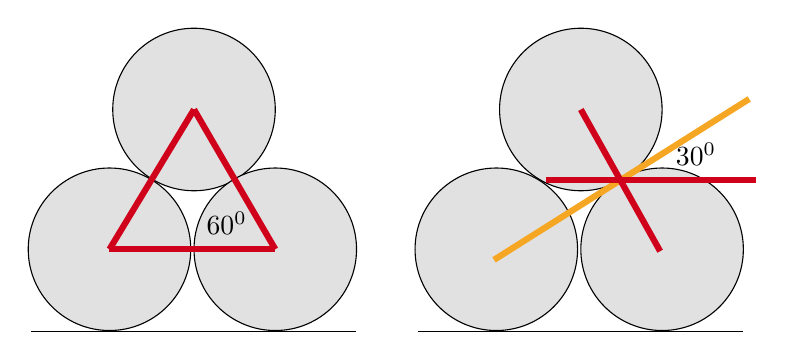
\begin{tikzpicture}[x=0.75pt,y=0.75pt,yscale=-0.7,xscale=0.7]
        %uncomment if require: \path (0,264); %set diagram left start at 0, and has height of 264

        %Shape: Ellipse [id:dp6454937638049347] 
        \draw  [fill={rgb, 255:red, 225; green, 225; blue, 225 }  ,fill opacity=1 ] (137.17,88.93) .. controls (137.17,58.04) and (162.21,33) .. (193.1,33) .. controls (224,33) and (249.04,58.04) .. (249.04,88.93) .. controls (249.04,119.82) and (224,144.87) .. (193.1,144.87) .. controls (162.21,144.87) and (137.17,119.82) .. (137.17,88.93) -- cycle ;
        %Shape: Ellipse [id:dp09659041693487258] 
        \draw  [fill={rgb, 255:red, 225; green, 225; blue, 225 }  ,fill opacity=1 ] (79,185.14) .. controls (79,154.25) and (104.04,129.21) .. (134.93,129.21) .. controls (165.82,129.21) and (190.87,154.25) .. (190.87,185.14) .. controls (190.87,216.03) and (165.82,241.07) .. (134.93,241.07) .. controls (104.04,241.07) and (79,216.03) .. (79,185.14) -- cycle ;
        %Shape: Circle [id:dp7523877018092493] 
        \draw  [fill={rgb, 255:red, 225; green, 225; blue, 225 }  ,fill opacity=1 ] (193.1,185.14) .. controls (193.1,154.25) and (218.15,129.21) .. (249.04,129.21) .. controls (279.93,129.21) and (304.97,154.25) .. (304.97,185.14) .. controls (304.97,216.03) and (279.93,241.07) .. (249.04,241.07) .. controls (218.15,241.07) and (193.1,216.03) .. (193.1,185.14) -- cycle ;
        %Straight Lines [id:da7934319805293468] 
        \draw    (80.79,241.52) -- (304.52,241.52) ;
        %Shape: Ellipse [id:dp9436597516501397] 
        \draw  [fill={rgb, 255:red, 225; green, 225; blue, 225 }  ,fill opacity=1 ] (403.41,88.93) .. controls (403.41,58.04) and (428.46,33) .. (459.35,33) .. controls (490.24,33) and (515.28,58.04) .. (515.28,88.93) .. controls (515.28,119.82) and (490.24,144.87) .. (459.35,144.87) .. controls (428.46,144.87) and (403.41,119.82) .. (403.41,88.93) -- cycle ;
        %Shape: Ellipse [id:dp5128552258927073] 
        \draw  [fill={rgb, 255:red, 225; green, 225; blue, 225 }  ,fill opacity=1 ] (345.24,185.14) .. controls (345.24,154.25) and (370.29,129.21) .. (401.18,129.21) .. controls (432.07,129.21) and (457.11,154.25) .. (457.11,185.14) .. controls (457.11,216.03) and (432.07,241.07) .. (401.18,241.07) .. controls (370.29,241.07) and (345.24,216.03) .. (345.24,185.14) -- cycle ;
        %Shape: Ellipse [id:dp21704569705186105] 
        \draw  [fill={rgb, 255:red, 225; green, 225; blue, 225 }  ,fill opacity=1 ] (459.35,185.14) .. controls (459.35,154.25) and (484.39,129.21) .. (515.28,129.21) .. controls (546.17,129.21) and (571.21,154.25) .. (571.21,185.14) .. controls (571.21,216.03) and (546.17,241.07) .. (515.28,241.07) .. controls (484.39,241.07) and (459.35,216.03) .. (459.35,185.14) -- cycle ;
        %Straight Lines [id:da9042183550203948] 
        \draw    (347.03,241.52) -- (570.77,241.52) ;
        %Straight Lines [id:da8134842484634719] 
        \draw [color={rgb, 255:red, 245; green, 166; blue, 35 }  ,draw opacity=1 ][line width=2.25]    (575.24,81.67) -- (399.61,192.42) ;
        %Straight Lines [id:da47693545074586075] 
        \draw [color={rgb, 255:red, 208; green, 2; blue, 27 }  ,draw opacity=1 ][line width=2.25]    (193.1,88.93) -- (134.93,185.14) ;
        %Straight Lines [id:da8341487281668398] 
        \draw [color={rgb, 255:red, 208; green, 2; blue, 27 }  ,draw opacity=1 ][line width=2.25]    (249.04,185.14) -- (134.93,185.14) ;
        %Straight Lines [id:da8027791787204905] 
        \draw [color={rgb, 255:red, 208; green, 2; blue, 27 }  ,draw opacity=1 ][line width=2.25]    (249.04,185.14) -- (193.1,88.93) ;
        %Straight Lines [id:da27035493326436333] 
        \draw [color={rgb, 255:red, 208; green, 2; blue, 27 }  ,draw opacity=1 ][line width=2.25]    (513.94,186.48) -- (459.35,88.93) ;
        %Straight Lines [id:da5901311794622432] 
        \draw [color={rgb, 255:red, 208; green, 2; blue, 27 }  ,draw opacity=1 ][line width=2.25]    (579.72,137.48) -- (435.41,137.48) ;

        % Text Node
        \draw (200,158) node [anchor=north west][inner sep=0.75pt]    {$60^0$};
        % Text Node
        \draw (523,110) node [anchor=north west][inner sep=0.75pt]    {$30^0$};


    \end{tikzpicture}

\end{figure}

\subsection{Projectile motion}
Range on plane inclined at angle $\phi$ is maximised when launch angle with respect to the plane, $\theta=(\pi/2-\phi)/2$ (along the angle bisector of the vertical and the plane).

One can show that the set of points a projectile can reach with some initial speed $v$ is a parabola with a focus at the launching point with equation
\begin{equation}
    y=\frac{v^2}{2g}-\frac{g}{2v^2}x^2
\end{equation}

A parabola is defined as a set of points where the distacne from the focus is the same as the distance from the directrix. This fact can be used to prove many things. The directrix of an envelope is a distance $d=1/4a$ from the turning point. 

\begin{enumerate}
    \item The final velocity of the projectile when it touches the envelope, $\mathbf{v_f}$ is perpendicular to the initial velocity $\mathbf{v_i}$.
    \item Since $\mathbf{v_f}$ is tangent to the envelope, it is along the angle bisector between the vertical and line from focus to the point. 
\end{enumerate}



\subsection{Minimisation}
To find the minimum value of some quantity, it is often useful to think about all possible values of that quantity. This can reveal a solution using geometry or symmetry. It is useful to also consider velocity space and space time to visualise the process. 

\subsection{Kinematics involving friction}
In problems with friction, the best reference frame to use is almost always the frame of whatever is causing the friction. 

\subsection{Rabbit and fox problem}
Problem can be solved by considering the rate of change of horizontal distance and rate of change of velocity vector that connects the rabbit and the fox. You will see that $r+x$ is conserved (very important fact).

\subsection{Non-inertial reference frames}
I think fictitious forces are just there to make sure that everything works on in non-inertial reference frames as well.

\subsubsection{Translational}
Let the lab frame be $S$, and the non inertial frame moving at $\vec{a_0}$ be $S'$. If the object's acceleration is $\vec{a}$ in the lab frame, its acceleration in the non-inertial frame would be $\vec{a}-\vec{a_0}=\vec{a'}$. The fictitious force present is thus $-m \vec{a_0}$. (translational force)

\subsubsection{Rotational}
Consider a system of reference, which rotates around the origin $O$ with an angular velocity $\boldsymbol{\omega}$. Consider a point $P$, which is motionless in the ortating system, and let us denote $\vec{r}=\vec{OP}$.
In the lab system of reference, the point $P$ moves with velocity $\mathbf{v}=\frac{d\mathbf{r}}{dt}=\mathbf{r} \times \boldsymbol{\omega}$. Now, if the point $P$ moves in the rotating frame of refernece with velocity $\mathbf{u}=\frac{d\mathbf{r}}{d\tau}$ ($\tau$ is used to emasure the time in the rotating system), then this additional velocity needs to be added to what should have been for a motionless point:
$$\frac{d\mathbf{r}}{dt}=\frac{d\mathbf{r}}{d\tau}+\boldsymbol{\omega}\times \mathbf{r}$$
So, we can conclude that the time-derivatives of vectors in rotating and lab frames of refernce are related via equality
$$\frac{d}{dt}=\frac{d\mathbf{r}}{d\tau}+\boldsymbol{\omega}\times . $$
This is written in the form of an operator, which means that we can write any vector (e.g. $\mathbf{r}$,$\mathbf{v}$) rightwards of all the three terms. In particular, we can apply this formula to the right and left hand sides of the equality $\mathbf{v}=\mathbf{u}+\boldsymbol{\omega} \times \mathbf{r}$

$$\frac{d\mathbf{v}}{dt}=\bigg(\frac{d}{d\tau}+\boldsymbol{\omega}\times\bigg)\bigg(\mathbf{u}+\boldsymbol{\omega}\times\mathbf{r}\bigg)
    \\
    = \frac{d\mathbf{u}}{d\tau}+\boldsymbol{\omega}\times\mathbf{u}+\frac{d(\boldsymbol{\omega}\times \mathbf{r})}{d\tau}+\boldsymbol{\omega}\times(\boldsymbol{\omega}\times \mathbf{r})$$
We obtain
$$\frac{d\mathbf{v}}{dt}=\frac{d\mathbf{u}}{d\tau}+2\boldsymbol{\omega}\times\mathbf{u}-\boldsymbol{\omega}^2\mathbf{r}$$

Recall that $\frac{d\mathbf{v}}{dt}$ is the acceleration of the point $P$ as seen in the lab frame of refernce, and $\frac{d\mathbf{u}}{d\tau}$ is the same as seen in the rotating frame of reference. now, if $P$ is a point mass $m$, and thee is an external force $\mathbf{F}$ acting on $P$, then $\mathbf{F}=m\frac{d\mathbf{v}}{dt}$ and hence,
\begin{equation}
    m\frac{d\mathbf{u}}{d\tau}=\mathbf{F}-2\boldsymbol{\omega}\times\mathbf{u}m+\boldsymbol{\omega}^2\mathbf{r}m
\end{equation}
\subsubsection{Unconventional method}
For rotating masses, we can work in the complex plane $r=x+iy$. The general solution for the path is 
\begin{equation}
    r(t)=r_0 + r_1 e^{i\omega_1 t}
\end{equation}
where $omega_1$ is the angular frequency \textbf{in} the rotating frame. 
To transform back to the lab frame, we just need to multiply by $e^{i\omega_0t}$, where $\omega_0$ is the angular frequency \textbf{of} the rotating frame.

\textcolor{blue}{In general, complex numbers are useful to deal with magnetic or Coriolis forces for motion in a plane. In these cases the force lies in a plane perpendicular to the velocity, so it's just proportional to $i\dot{r}$.}

\section{Friction}
\subsection{Friction on inclined slope}
If a body is on the verge of slipping (or already slipping), then the sum of the friction force and the reaction force is angled by $\arctan{\mu}$ from the surface normal. This is actually quite useful in certain questions. \textcolor{blue}{\textit{Sometimes, we don't even have to resolve forces by projecting their components onto axes. We can instead add them up vectorially by drawing vector diagram (head to tail).}} This can be shown in the example below from \textit{Jaan Kalda's Mechanics handout}.

\begin{mybox}{gray}{Mechanics \textbf{pr 5.}}
    \begin{wrapfigure}{l}{0.6\textwidth}
        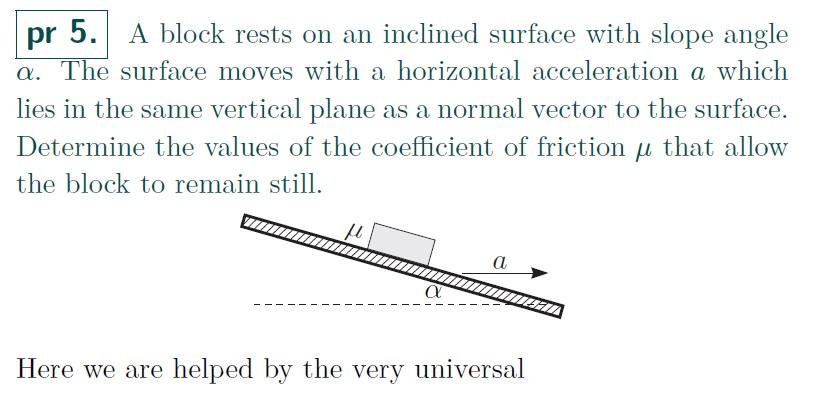
\includegraphics[scale=0.5]{pr 5.jpg}
    \end{wrapfigure}

    \textbf{Method 1} \quad
    To solve this problem, the common method would be to resolve forces
    Resolving forces along the slope gives us:
    $$mg\sin\alpha-f-ma\cos\alpha=0$$
    Resolving forces perpendicular to the slope gives us:
    $$N-mg\cos\alpha-ma\sin\alpha=0$$
    Since $N$ must be positive for the block to stay on the plane, we get the first inequality
    $$g\cos\alpha+a\sin\alpha > 0$$
    Our second inequality comes from the force balance along the slope, where $\mid f \mid\leq\mu N$
    So we get
    \begin{equation}
        \mu \geq \frac{\mid a\cos\alpha-g\sin\alpha \mid}{g\cos\alpha+a\sin\alpha}
    \end{equation}
    Both inequalities have to be satisfied for the block to remain on the slope.
\end{mybox}



\section{Tension}
\subsection{Rubber band around cylinder}
In fact, we have to
\begin{enumerate}
    \item Analyse an infinitesimal string element which subtends an angle of $d\theta$.
    \item It is not hard to see that the radial component is $T\sin\frac{d\theta}{2}$. By small angle approximation, which states that $sin\theta \approx \theta$ for small $\theta$, we get: $Td\theta$ (2 tensions acting on both ends)
    \item Integrate this tension from $0$ to $2 \pi $, the total tension would then be (look abit weird but I think it's correct) $2 \pi T$.
\end{enumerate}

\subsection{Hanging Chain}
\begin{mybox}{gray}{Example from \textbf{Morin 2.8}}
    \begin{enumerate}
        \item Realise that $T_x$ is constant throughout the chain, and $\frac{T_y}{T_x}=y'$. Hence, $T_y=T_x y' = C y'$
        \item And also realised that the mass of each infinitesimal chain segments can be expressed as such
              \begin{equation}
                  \rho \vec{g} dl= \rho \vec{g} \sqrt {dx^2+dy^2}=\rho \vec{g} \sqrt {1+y'^2}dx
              \end{equation}
        \item However, it is the \textbf{difference in tension} that balance out the wright. We can then write down the final relationships and solve the equation using substitution and separation of variables.
              \begin{equation}
                  d(Cy')= \rho \vec{g} \sqrt {1+y'^2}dx
              \end{equation}
              \begin{equation}
                  C y''= \rho \vec{g} \sqrt {1+y'^2}
              \end{equation}
    \end{enumerate}
\end{mybox}

\section{SHM}
\subsection{Translational perturbation}
\begin{enumerate}
    \item Find $\sum F$, and find all the equilibrium positions where $\sum F=0$ (these are the stable equilibriums)
    \item Use: $k=-\frac{dF}{dx}$. (negative sign depends on the direction of F. In this case, F is defined as positive in the direction that points away from equilibrium)
    \item Then do smth like $\frac{dF}{dx}\big|_{x=x_{\textsf{eqm}}}$, and substitute the values (Hookes constant $k$) into $\omega = \sqrt \frac{k}{m}$
\end{enumerate}

\subsection{Radial perturbation}
I am not sure about this, but this is what i see people do on PhOD to solve questions (physics olympiad discord)
\begin{enumerate}
    \item Let the small perturbation "displacement" be $\delta$.
    \item If the mass is revolving around some bigger object and the only force acting on it is in the radial direction, then we can use \textbf{conservation of angular momentum}
          \begin{equation}
              r^2\omega=(r+\delta)^2\omega'
          \end{equation}
          Through simple algebraic manipulation, we get
          \begin{equation}
              \omega'= \bigg(\frac{r}{r+\delta}\bigg)^2\omega
          \end{equation}
    \item In the rotating frame, we can write
          \begin{equation}
              m \frac{d^2 \delta}{dt^2}= m (r+\delta)\omega'^2-F_{\textsf{central}}
          \end{equation}
    \item Try to fit that to the classic SHM equation (maybe can simplify RHS and expand to first order in $\delta$): $\ddot{x}+\omega^2 x = 0$, and use $\omega = \sqrt \frac{k}{m}$
\end{enumerate}

\section{SJPO2021 Special Round Qn}
\begin{mybox}{gray}{Da question}

    \begin{wrapfigure}{l}{0.4\textwidth}
        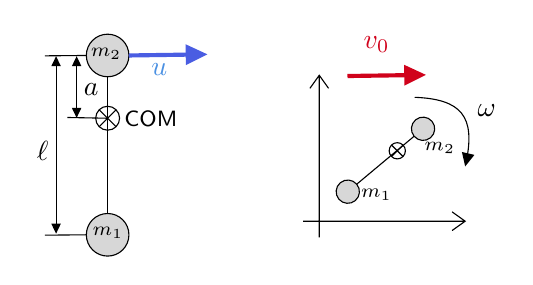
\begin{tikzpicture}[x=0.75pt,y=0.75pt,yscale=-0.9,xscale=0.9]
            %uncomment if require: \path (0,300); %set diagram left start at 0, and has height of 300

            %Shape: Circle [id:dp19822565348906274] 
            \draw  [fill={rgb, 255:red, 215; green, 215; blue, 215 }  ,fill opacity=1 ] (149,40.4) .. controls (149,34.1) and (154.1,29) .. (160.4,29) .. controls (166.7,29) and (171.8,34.1) .. (171.8,40.4) .. controls (171.8,46.7) and (166.7,51.8) .. (160.4,51.8) .. controls (154.1,51.8) and (149,46.7) .. (149,40.4) -- cycle ;
            %Shape: Circle [id:dp3426728199976101] 
            \draw  [fill={rgb, 255:red, 215; green, 215; blue, 215 }  ,fill opacity=1 ] (149,136.4) .. controls (149,130.1) and (154.1,125) .. (160.4,125) .. controls (166.7,125) and (171.8,130.1) .. (171.8,136.4) .. controls (171.8,142.7) and (166.7,147.8) .. (160.4,147.8) .. controls (154.1,147.8) and (149,142.7) .. (149,136.4) -- cycle ;
            %Straight Lines [id:da8938425234356642] 
            \draw    (160.4,51.8) -- (160.4,125) ;
            %Straight Lines [id:da6191489683695304] 
            \draw [color={rgb, 255:red, 74; green, 93; blue, 226 }  ,draw opacity=1 ][line width=1.5]    (171.8,40.4) -- (205.83,39.91) -- (209.8,39.86) ;
            \draw [shift={(213.8,39.8)}, rotate = 539.1800000000001] [fill={rgb, 255:red, 74; green, 93; blue, 226 }  ,fill opacity=1 ][line width=0.08]  [draw opacity=0] (11.61,-5.58) -- (0,0) -- (11.61,5.58) -- cycle    ;
            %Shape: Axis 2D [id:dp15146894469957406] 
            \draw  (265,129.12) -- (351.8,129.12)(273.68,51) -- (273.68,137.8) (344.8,124.12) -- (351.8,129.12) -- (344.8,134.12) (268.68,58) -- (273.68,51) -- (278.68,58)  ;
            %Straight Lines [id:da5814568840159711] 
            \draw [color={rgb, 255:red, 208; green, 2; blue, 27 }  ,draw opacity=1 ][line width=1.5]    (288.8,51.4) -- (322.83,50.91) -- (326.8,50.86) ;
            \draw [shift={(330.8,50.8)}, rotate = 539.1800000000001] [fill={rgb, 255:red, 208; green, 2; blue, 27 }  ,fill opacity=1 ][line width=0.08]  [draw opacity=0] (11.61,-5.58) -- (0,0) -- (11.61,5.58) -- cycle    ;
            %Shape: Circle [id:dp4673346981336375] 
            \draw  [fill={rgb, 255:red, 215; green, 215; blue, 215 }  ,fill opacity=1 ] (325.26,74.86) .. controls (327.9,72.65) and (331.84,73.01) .. (334.04,75.65) .. controls (336.25,78.29) and (335.9,82.22) .. (333.26,84.43) .. controls (330.61,86.64) and (326.68,86.29) .. (324.47,83.64) .. controls (322.27,81) and (322.62,77.07) .. (325.26,74.86) -- cycle ;
            %Shape: Circle [id:dp48839595309985206] 
            \draw  [fill={rgb, 255:red, 215; green, 215; blue, 215 }  ,fill opacity=1 ] (284.96,108.53) .. controls (287.61,106.32) and (291.54,106.68) .. (293.75,109.32) .. controls (295.96,111.96) and (295.6,115.89) .. (292.96,118.1) .. controls (290.32,120.31) and (286.38,119.96) .. (284.18,117.32) .. controls (281.97,114.67) and (282.32,110.74) .. (284.96,108.53) -- cycle ;
            %Straight Lines [id:da5712778086817507] 
            \draw    (324.47,83.64) -- (293.75,109.32) ;
            %Flowchart: Summing Junction [id:dp33175257463483754] 
            \draw   (154,74) .. controls (154,70.47) and (156.87,67.6) .. (160.4,67.6) .. controls (163.93,67.6) and (166.8,70.47) .. (166.8,74) .. controls (166.8,77.53) and (163.93,80.4) .. (160.4,80.4) .. controls (156.87,80.4) and (154,77.53) .. (154,74) -- cycle ; \draw   (155.87,69.47) -- (164.93,78.53) ; \draw   (164.93,69.47) -- (155.87,78.53) ;
            %Flowchart: Summing Junction [id:dp6201575245730861] 
            \draw   (311.11,91.43) .. controls (311.11,89.03) and (313.06,87.08) .. (315.46,87.08) .. controls (317.85,87.08) and (319.8,89.03) .. (319.8,91.43) .. controls (319.8,93.83) and (317.85,95.77) .. (315.46,95.77) .. controls (313.06,95.77) and (311.11,93.83) .. (311.11,91.43) -- cycle ; \draw   (312.38,88.35) -- (318.53,94.5) ; \draw   (318.53,88.35) -- (312.38,94.5) ;
            %Straight Lines [id:da03269001228001933] 
            \draw    (126.8,40.6) -- (149,40.4) ;
            %Straight Lines [id:da1122374457863542] 
            \draw    (138.8,73.6) -- (160.4,74) ;
            %Straight Lines [id:da009815337614956343] 
            \draw    (126.8,136.6) -- (149,136.4) ;
            %Straight Lines [id:da44886965522336975] 
            \draw    (143.8,43.8) -- (143.8,70.8) ;
            \draw [shift={(143.8,73.8)}, rotate = 270] [fill={rgb, 255:red, 0; green, 0; blue, 0 }  ][line width=0.08]  [draw opacity=0] (5.36,-2.57) -- (0,0) -- (5.36,2.57) -- cycle    ;
            \draw [shift={(143.8,40.8)}, rotate = 90] [fill={rgb, 255:red, 0; green, 0; blue, 0 }  ][line width=0.08]  [draw opacity=0] (5.36,-2.57) -- (0,0) -- (5.36,2.57) -- cycle    ;
            %Straight Lines [id:da577760339017418] 
            \draw    (132.8,43.8) -- (132.8,132.8) ;
            \draw [shift={(132.8,135.8)}, rotate = 270] [fill={rgb, 255:red, 0; green, 0; blue, 0 }  ][line width=0.08]  [draw opacity=0] (5.36,-2.57) -- (0,0) -- (5.36,2.57) -- cycle    ;
            \draw [shift={(132.8,40.8)}, rotate = 90] [fill={rgb, 255:red, 0; green, 0; blue, 0 }  ][line width=0.08]  [draw opacity=0] (5.36,-2.57) -- (0,0) -- (5.36,2.57) -- cycle    ;
            %Curve Lines [id:da5841429723653924] 
            \draw    (324.8,62.8) .. controls (349.89,63.77) and (357.29,73.11) .. (352.38,97.13) ;
            \draw [shift={(351.8,99.8)}, rotate = 282.99] [fill={rgb, 255:red, 0; green, 0; blue, 0 }  ][line width=0.08]  [draw opacity=0] (7.14,-3.43) -- (0,0) -- (7.14,3.43) -- cycle    ;

            % Text Node
            \draw (162.4,135.4) node  [font=\scriptsize]  {$m_{1\ }$};
            % Text Node
            \draw (125.62,91.4) node    {$\mathrm{\ell }$};
            % Text Node
            \draw (182.4,43.3) node [anchor=north west][inner sep=0.75pt]  [color={rgb, 255:red, 74; green, 144; blue, 226 }  ,opacity=1 ]  {$u$};
            % Text Node
            \draw (161.4,39.4) node  [font=\scriptsize]  {$m_{2\ }$};
            % Text Node
            \draw (304.37,34.76) node  [color={rgb, 255:red, 74; green, 144; blue, 226 }  ,opacity=1 ]  {$\textcolor[rgb]{0.82,0.01,0.11}{v_{0}}$};
            % Text Node
            \draw (306.08,114.81) node  [font=\scriptsize,rotate=-359.24]  {$m_{1\ }$};
            % Text Node
            \draw (340.03,89.72) node  [font=\scriptsize,rotate=-1.09]  {$m_{2\ }$};
            % Text Node
            \draw (151.62,58.4) node    {$a$};
            % Text Node
            \draw (168,69) node [anchor=north west][inner sep=0.75pt]   [align=left] {{\fontfamily{cmss}\selectfont {\footnotesize COM}}};
            % Text Node
            \draw (363.37,69.76) node  [color={rgb, 255:red, 74; green, 144; blue, 226 }  ,opacity=1 ]  {$\textcolor[rgb]{0,0,0}{\mathbf{\omega }}$};
        \end{tikzpicture}
    \end{wrapfigure}

    Basically the question asks you to find the equation for the trajectory of the thing shown in the diagram when $m_2$ starts with an initial velocity $u$ perpendicular to the rod. (masses on frictionless ground). I think using the centre of mass frame would help in solving this problem.
    \hfill
\end{mybox}
Position of centre of mass with respect to $m_2$,
\begin{equation}
    a=\frac{m_1 \ell}{m_1+m_2}
\end{equation}
Velocity of centre of mass of the system can be calculated through conservation of momentum:
\begin{equation}
    v_{\textsf{COM}}=\frac{m_2u}{m_1+m_2}
\end{equation}
The moment of inertia of the system with respect to its centre of mass is
\begin{equation}
    I=m_2 \bigg(\frac{m_1 \ell}{m_1+m_2}\bigg)^2+m_1\bigg(\frac{m_2 \ell}{m_1+m_2}\bigg)^2=\frac{m_1 m_2 \ell^2}{m_1+m_2}
\end{equation}
Angular velocity could be either determined using \textbf{angular momentum}:
\begin{equation}
    \omega=\frac{L}{I}
\end{equation}
\begin{equation}
    \therefore\omega=\frac{u}{\ell}
\end{equation}
Or determined by \textbf{finding velocity of $m_2$ in the COM frame} and then \textbf{divide by the radius of rotation to find angular velocity} as $v=r\omega$.
\begin{equation}
    v'=u-\frac{m_2 u}{m_1+m_2}=\frac{m_1 u}{m_1+m_2}
\end{equation}
Dividing this by the radius of rotation (distance from $m_2$ to COM), we obtain the same expression for $\omega$
\begin{equation}
    \omega= \frac{v'}{a}=\frac{u}{\ell}
\end{equation}

Formulating the equation for trajectory:
\begin{equation}
    x(t)=a \sin (-\omega t)+v_{\textsf{COM}}t
\end{equation}
\begin{equation}
    y(t)=a \cos(\omega t)
\end{equation}
\begin{figure}[H]
    \centering
    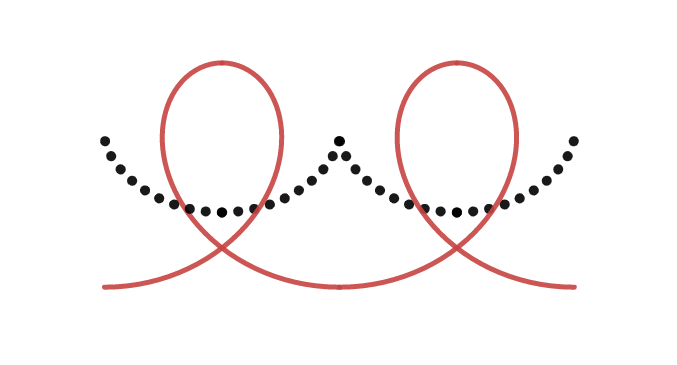
\includegraphics[width=10cm]{graph latex.jpeg}
    \caption{Trajectory plotted with Desmos}
    \label{fig:2}
\end{figure}

\section{Gravitation}
\section{Scaling and Parallel Axis theorem}
\subsection{MOI of a sierpinski triangle}

\def\trianglewidth{2cm}%
\pgfdeclarelindenmayersystem{Sierpinski triangle}{
    \symbol{X}{\pgflsystemdrawforward}
    \symbol{Y}{\pgflsystemdrawforward}
    \rule{X -> X-Y+X+Y-X}
    \rule{Y -> YY}
}
\foreach \level in {0,...,6}{
\tikzset{
    l-system={step=\trianglewidth/(2^\level), order=\level, angle=-120}
}
\begin{tikzpicture}
        \fill [black] (0,0) -- ++(0:\trianglewidth) -- ++(120:\trianglewidth) -- cycle;
        \draw [draw=none] (0,0) l-system
        [l-system={Sierpinski triangle, axiom=X},fill=white];
\end{tikzpicture}
}

\subsubsection{Building up}
We will build the triangle from the smallest triangle possible, and slowly work backwards. Let the smallest triangle be the basic repeating unit with mass $m$ and side length $\ell$. 

It is obvious that $m_{n+1}=3m_n$ and $\ell_{n+1}=2\ell_n$ with $I_{n+1}=3(I_n+m a^2)=3I_n+m\ell_n^2$ where a is the distance from the COM of the small triangle to that of the big triangle and is $\ell_n/\sqrt{3}$

The moment inertia can then be found through iterations,
\begin{align}
    I_1 
    &= 3Cm_0\ell_0^2+m_0^2\ell_0^2 = (3C+1)m_0\ell_0^2\nonumber\\
    I_2 &= 3I_1+m_1\ell_1^2=(3^2C+3+12)m_0\ell_0^2\nonumber\\
    I_3 &= 3I_2+m_2\ell_2^2=(3^2C+3^2+3\time 12+12^2)m_0\ell_0^2\nonumber\\
    I_n &= 3I_{n-1}+m_{n-1}\ell_{n-1}^2=(12^{n-1}+12^{n-2}3+...+3^{n-1}+3^n C)m_0\ell_0^2
\end{align}
where $Cm_0\ell_0^2$ is the moment of inertia of the basic building block

Taking the limits as $n\to\infty$
\begin{equation}
    \lim_{n\to\infty}I_n=12^{n-1}m_0\ell_0^2\bigg(1+\frac{1}{4}+\frac{1}{4^2}+...+\frac{1}{4^{n-1}}+\frac{1}{4^n}C\bigg)
\end{equation}
We note that the last term with $C$ plays no role in this infinite geometric series. After defining $\lim_{n\to\infty} 3^n m_0=M $ and $\lim_{n\to\infty} 2^n \ell_0=\ell$, and simplifying the above expression, we get

\begin{equation}
    \lim_{n\to\infty}I_n=\frac{1}{9}M\ell^2
\end{equation}

\subsubsection{Repeating pattern}
For a 2D-planar object (this is also from Ryan's lesson), the moment of inertia is calculated using 
\begin{equation}
    I=\int r^2 dm =\int r^2 \sigma dx dy
\end{equation}

where $\sigma$ is the surface mass density. We see that if we were to scale the side length of the planar object by 2 (or just scale it up by 2 times), the moment of inertia will be scaled up by $2^2 \times 2 \times 2=16$, due to the $r^2 dx dy$ in the above integral. 

However, the tricky part is that for a sierpinski triangle, it is a bit different. Because the $\sigma$ is always changing. Instead, we can rewrite $I$ as 
\begin{equation}
    I=\int r^2 dm
\end{equation}
If we were to scale up the triangle by 2 (go up by 1 layer), $r^2 dm$ will be equivalent to scaling $I$ up by $2^2 \times 3= 12$ times. 

so let the moment of inertia of one infinite siepinski triangle be $I$ with side length $\ell$. We know that we can form a bigger siepinski triangle (side length: $2\ell$) with 3 smaller ones. With this method, we arrive at the same answer
\begin{align}
    (2^2\times 3) I &= 3I+ m \ell^2\\
    I&=\frac{1}{9}m \ell^2
\end{align}

\subsection{Limitation of PAT}
It only works if the initial moment of inertia is calculated about the object's centre of mass. (how did I not know this gosh)
\begin{equation}
    I=I_{\textsf{cm}}+md^2
\end{equation}


ohhhhhh penguinnn
\begin{figure}[htbp]
    \centering
    
\begin{tikzpicture}
        \penguin
    \end{tikzpicture}
\end{figure}

\section{Torque}
\subsection{Generally speaking...}
The method where you prove $\sum\tau=0$ by extending lines of action (LOA) of the object and make sure they intersect, \textbf{it only works for a group of 2/3 forces}. So let's say if you have $5$ forces in total, to make the net torque 0, the LOA of 2 of the forces intersect at one point, while the LOA of the remaining 3 forces intersect at another point. (lmao learn something new everyday)

If the total force vanishes, the total torque about any point is 0. If the total force is not 0, then this is no longer the case. 
\subsection{Tilting and hanging objects}
\begin{enumerate}
    \item For an object to not tilt, the \textbf{COM must be directly above the contact point}. 
    \item For an object hung on the string in equilibrium, the \textbf{COM is always directly below the string attachment point}.
\end{enumerate}


\chapter{Electromagnetism}

\section{Electric field and potential}
Potential and field are related by the following equation
\begin{equation}
    -\int_A^B E \cdot ds = V(B)-V(A)
\end{equation}
I think the intuition is that a \textbf{positive workdone by E field} always results in a decrease in \textbf{potential}.

\begin{mybox}{green}{Intuition}
    when the E field is pointing away from a \textbf{positive charge}, to move the \textbf{negative test charge} away from the positive charge, you need a force with magnitude of at least $qE$ and opposite in direction of the force of attraction. Workdone by that force results in an increase in potential (less negative) by conservation of energy. Since $Eq$ always points in the opposite direction of that force, $qE$ always points in direction of decreasing potential.
\end{mybox}
\subsection{Faraday's law of induction}
\subsection{More about electromotive force}

In the circuit, the flowing electrons experience 2 forces, namely the force provided by the external agent, such as the battery ($\vec{f_s}$), and the force provided by E-field due to the build-up of charges around the circuit ($\vec{E}$).

Hence, the net force driving the current is
\begin{equation}
    \vec{f}=\vec{f_s}+\vec{E}
\end{equation}
The emf (electromotive force) is defined as
\begin{equation}
    \textsf{emf}=\oint \mathbf{f} \cdot d\mathbf{s}=\oint \mathbf{f_s} \cdot d\mathbf{s}
\end{equation}
This is because $\oint \mathbf{E} \cdot d\mathbf{s}=0$.


\section{Different kinds of "Current"}
\subsubsection{linear current}
\begin{equation}
    \mathbf{I}=\lambda \mathbf{v}
\end{equation}
The unit for $\lambda$ is $[A][m]^{-1}[s]$.
This seemed a bit weird to be initially. I guess can think about it this way:
\begin{mybox}{green}{I guess this makes sense...}
    \begin{equation}
        \mathbf{I}=\frac{Q}{t}
    \end{equation}
    \begin{equation}
        \mathbf{I}=\frac{\lambda d}{t}=\lambda \mathbf{v}
    \end{equation}
\end{mybox}
\subsubsection{surface current}
\begin{equation}
    \mathbf{K}=\frac{d\mathbf{I}}{d\ell_\perp}=\sigma \mathbf{v}
\end{equation}
The unit for $\sigma$ is $[A][m]^{-2}[s]$
\subsubsection{volume current}
\begin{equation}
    \mathbf{J}=\frac{d\mathbf{I}}{da_\perp}=\rho \mathbf{v}
\end{equation}
\section{Vector potential is pretty gae}

\begin{proof}[Vector potential]
    In electrostatics, we have $-\nabla \mathbf{V}=\mathbf{E}$, thanks to the fact that $\nabla \times \mathbf{V}=0$.
    Apparently, we can also define such a potential ($\mathbf{V}$) for magnostatics ($\mathbf{A}$).
    Since $\nabla \cdot \mathbf{B}=0$, it allows for $\nabla \times \mathbf{A}=\mathbf{B}$ (divergence of curl: $\nabla \cdot \mathbf{B}=\nabla \cdot (\nabla \times \mathbf{A})=0$)

    We can substitute $\nabla \times \mathbf{A}=\mathbf{B}$ into $\nabla \times \mathbf{B}$, and get

    \begin{eqnarray}
        \nabla \times (\nabla \times \mathbf{A})&=&\nabla(\nabla \cdot \mathbf{A})-\nabla \cdot (\nabla \mathbf{A})\\
        &=&\nabla(\nabla \cdot \mathbf{A})-\nabla^2 \mathbf{A}=\mu_0 \mathbf{J}
    \end{eqnarray}

    But why are we doing this? Well, if we can make $\nabla(\nabla \cdot \mathbf{A})=0$, then we get $-\nabla^2 \mathbf{A}=\mu_0 \mathbf{J}$ (just \textbf{Poisson's equation}), making the magnetic vector potential a very useful tool, from which the B field can then be easily calculated.

    To show that we can indeed obtain \textbf{Poisson's equation} for magnetism, we now have to prove that it is possible to let $\nabla \cdot \mathbf{A}=0$.

    Supposed the original $\mathbf{A_0}$ is not divergenceless. But we can make it divergenceless by adding the \textbf{gradient} of something else, maybe $\nabla \mathbf{\Gamma}$ ($\mathbf{\Gamma}$ looks cool), turning $\mathbf{A_0}$ into $\mathbf{A}$.We are adding the gradient of something else because we don't want it to affect $\nabla \times \mathbf{A}$, since the curl of gradient is 0 (so the curl is still $\mathbf{B}$). We then get
    \begin{equation}
        \nabla \cdot \mathbf{A}=\nabla \cdot \mathbf{A_0}+\nabla ^2 \mathbf{\Gamma}
    \end{equation}
    Setting $\nabla \cdot \mathbf{A}=0$, we get
    \begin{equation}
        \nabla \cdot \mathbf{A_0}=-\nabla ^2 \mathbf{\Gamma}
    \end{equation}
    This is again, just Poisson's equation, and we know that there will always be a solution for $\mathbf{\Gamma}$. Hence, it is always possible to make $\mathbf{A}$ divergenceless while still keeping $\nabla \times \mathbf{A}=\mathbf{B}$.
    \begin{equation}
        \boxed{\nabla^2 \mathbf{A}=-\mu_0 \mathbf{J}}\qedhere
    \end{equation}
\end{proof}

\section{Dipoles}
\subsection{Electric dipole}
Torque experienced by electric dipole in a uniform electric field is
\begin{equation}
    \mathbf{N}=\mathbf{p} \times \mathbf{E}
\end{equation}
The equation for force experienced by an electric dipole is given by $mathbf{F}=\nabla(\mathbf{p} \cdot \mathbf{E})$ (used for non uniform $\mathbf{E}$ field), where $\mathbf{p}=qd$. It the E field is uniform, the net force would be 0, but the net torque would not be 0.

\begin{equation}
    \mathbf{F}=\nabla(\mathbf{p} \cdot \mathbf{E})=(\mathbf{p} \cdot \nabla)\mathbf{E}.
\end{equation}

\subsection{Magnetic dipole}
Torque experienced by a magnetic dipole in a uniform magnetic field is
\begin{equation}
    \mathbf{N}=\mathbf{m}\times \mathbf{B}
\end{equation}
The equation for force experienced by a magnetic dipole in \textbf{uniform magnetic field} is always 0.
\begin{mybox}{green}{Proof}
    The loop can be arranged/positioned in any manner in the uniform $\mathbf{B}$ field.
    The force on an infinitesimal part of the loop of length $d\ell$ is
    \begin{equation}
        d\mathbf{F}=(\mathbf{B} \times d\mathbf{l})I
    \end{equation}
    If we integrate the equation above around the loop, we get
    \begin{equation}
        \mathbf{F}=\mathbf{B}I\times\oint d\mathbf{l}
    \end{equation}
    where $\oint d\mathbf{l}=0$
\end{mybox}
In a non-uniform magnetic field, the force experienced would be
\begin{equation}
    \mathbf{F}=\nabla(\mathbf{m}\cdot \mathbf{B})
\end{equation}
Unlike the equation for electric dipole, $\mathbf{F} \neq (\mathbf{m}\cdot \nabla)\mathbf{B}$ (not sure why yet).

\subsection{Diamagnetism and Paramagnetism}
Paramagnets acquire a magnetisation parallel to $\mathbf{B}$ while diamagnets acquire a magnetisation opposite to $\mathbf{B}$. We will have to study the effect of magnetic field at the sub-atomic level...

\begin{mybox}{red}{Magnetic field and electron orbital}
    \begin{center}
        \tikzset{every picture/.style={line width=0.75pt}} %set default line width to 0.75pt        

        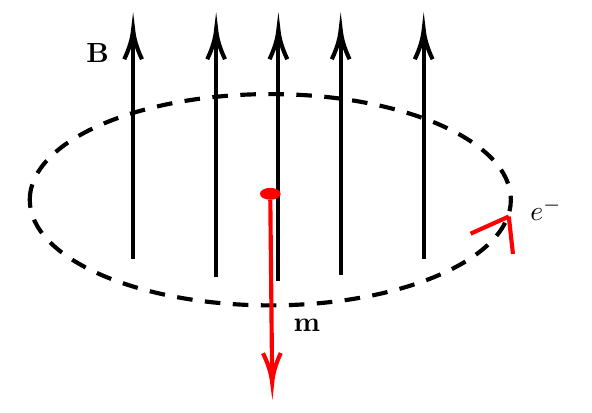
\begin{tikzpicture}[x=0.75pt,y=0.75pt,yscale=-1,xscale=1]
            %uncomment if require: \path (0,300); %set diagram left start at 0, and has height of 300

            %Shape: Ellipse [id:dp8639813058390806] 
            \draw  [dash pattern={on 5.63pt off 4.5pt}][line width=1.5]  (190,122.1) .. controls (190,93.99) and (241.89,71.2) .. (305.9,71.2) .. controls (369.91,71.2) and (421.8,93.99) .. (421.8,122.1) .. controls (421.8,150.21) and (369.91,173) .. (305.9,173) .. controls (241.89,173) and (190,150.21) .. (190,122.1) -- cycle ;
            %Straight Lines [id:da903094079444487] 
            \draw [line width=1.5]    (339.8,158.44) -- (339.8,43.2) ;
            \draw [shift={(339.8,40.2)}, rotate = 450] [color={rgb, 255:red, 0; green, 0; blue, 0 }  ][line width=1.5]    (14.21,-4.28) .. controls (9.04,-1.82) and (4.3,-0.39) .. (0,0) .. controls (4.3,0.39) and (9.04,1.82) .. (14.21,4.28)   ;
            %Straight Lines [id:da8758986216628213] 
            \draw [line width=1.5]    (279.8,159.44) -- (279.8,43.2) ;
            \draw [shift={(279.8,40.2)}, rotate = 450] [color={rgb, 255:red, 0; green, 0; blue, 0 }  ][line width=1.5]    (14.21,-4.28) .. controls (9.04,-1.82) and (4.3,-0.39) .. (0,0) .. controls (4.3,0.39) and (9.04,1.82) .. (14.21,4.28)   ;
            %Straight Lines [id:da2789297257171335] 
            \draw [line width=1.5]    (309.8,161.44) -- (309.8,43.2) ;
            \draw [shift={(309.8,40.2)}, rotate = 450] [color={rgb, 255:red, 0; green, 0; blue, 0 }  ][line width=1.5]    (14.21,-4.28) .. controls (9.04,-1.82) and (4.3,-0.39) .. (0,0) .. controls (4.3,0.39) and (9.04,1.82) .. (14.21,4.28)   ;
            %Straight Lines [id:da41807307836230745] 
            \draw [line width=1.5]    (239.8,150.44) -- (239.8,43.2) ;
            \draw [shift={(239.8,40.2)}, rotate = 450] [color={rgb, 255:red, 0; green, 0; blue, 0 }  ][line width=1.5]    (14.21,-4.28) .. controls (9.04,-1.82) and (4.3,-0.39) .. (0,0) .. controls (4.3,0.39) and (9.04,1.82) .. (14.21,4.28)   ;
            %Straight Lines [id:da9769541952675111] 
            \draw [line width=1.5]    (379.8,150.44) -- (379.8,43.2) ;
            \draw [shift={(379.8,40.2)}, rotate = 450] [color={rgb, 255:red, 0; green, 0; blue, 0 }  ][line width=1.5]    (14.21,-4.28) .. controls (9.04,-1.82) and (4.3,-0.39) .. (0,0) .. controls (4.3,0.39) and (9.04,1.82) .. (14.21,4.28)   ;
            %Straight Lines [id:da07955449336800569] 
            \draw [color={rgb, 255:red, 255; green, 0; blue, 0 }  ,draw opacity=1 ][line width=1.5]    (420.8,130.2) -- (402.4,138.44) ;
            %Straight Lines [id:da5605227952576148] 
            \draw [color={rgb, 255:red, 255; green, 0; blue, 0 }  ,draw opacity=1 ][line width=1.5]    (420.8,130.2) -- (422.8,148.2) ;
            %Straight Lines [id:da6729736350118587] 
            \draw [color={rgb, 255:red, 255; green, 0; blue, 0 }  ,draw opacity=1 ][line width=1.5]    (305.9,122.1) -- (306.77,207.2) ;
            \draw [shift={(306.8,210.2)}, rotate = 269.40999999999997] [color={rgb, 255:red, 255; green, 0; blue, 0 }  ,draw opacity=1 ][line width=1.5]    (14.21,-4.28) .. controls (9.04,-1.82) and (4.3,-0.39) .. (0,0) .. controls (4.3,0.39) and (9.04,1.82) .. (14.21,4.28)   ;
            %Shape: Ellipse [id:dp6844851006236772] 
            \draw  [draw opacity=0][fill={rgb, 255:red, 255; green, 0; blue, 0 }  ,fill opacity=1 ] (300.9,119.24) .. controls (300.9,120.82) and (303.14,122.1) .. (305.9,122.1) .. controls (308.66,122.1) and (310.9,120.82) .. (310.9,119.24) .. controls (310.9,117.66) and (308.66,116.39) .. (305.9,116.39) .. controls (303.14,116.39) and (300.9,117.66) .. (300.9,119.24) -- cycle ;

            % Text Node
            \draw (216,45.4) node [anchor=north west][inner sep=0.75pt]    {$\mathbf{B}$};
            % Text Node
            \draw (315.9,178.4) node [anchor=north west][inner sep=0.75pt]    {$\mathbf{m}$};
            % Text Node
            \draw (429.9,120.4) node [anchor=north west][inner sep=0.75pt]    {$e^{-}$};


        \end{tikzpicture}

    \end{center}

    Paramagnetism arises when the dipole moment\footnote{Fingers grip around direction of current (movement of \textbf{positive} charges, direction of thumb is the direction of dipole moment) - Right Hand Grip Rule} of the electron orbital align with the external magnetic field, while diamagnetism is a result of the change in the speed of electron due to the external magnetic field. The orbital contribution to paramagnetism is a lot smaller as it is much harder to tilt the orbital then to change its spin.

    The motion of the electron can be approximated as a steady current (because the orbital period is extremely short), then the magnetic dipole can be written as
    \begin{equation}
        \mathbf{m}=I\pi R^2 \hat{z}= \frac{-e}{T}\pi R^2 \hat{z} =\frac{-ev}{2\pi R}\pi R^2 \hat{z}=\frac{-evR}{2}\hat{z}
    \end{equation}
    where $R$ is the radius of the orbit (the negative sign accounts for the negative charge of the electron, as current is always a positive quantity)(v is defined as positive when it is anti clockwise).

    This shows that the electron orbital will always be subject to a torque ($\mathbf{m} \times \mathbf{B}$). However, it is hard to tilt the orbital. A more significant effect would be the change in speed of the electron due to the external $\mathbf{B}$ field.

    Assuming uniform circular motion, the initial speed ($v_0$) is given by
    \begin{equation}
        m \frac{v_0^2}{R}=\frac{1}{4\pi\epsilon_0}\frac{e^2}{R^2}
    \end{equation}

    Let's assume that the  $\mathbf{B}$ field is perpendicular to the orbit, the new speed of the electron would be given by
    \begin{equation}
        m \frac{v_1^2}{R^2}=\frac{1}{4\pi\epsilon_0}\frac{e^2}{R^2}+ev_1B
    \end{equation}
    \begin{equation}
        ev_1B=\frac{m}{R}(v_1^2-v_0^2)=\frac{m}{R}(v_1-v_0)(v_1+v_0)=\frac{m}{R}(\Delta v)(v_1+v_0)
    \end{equation}
    Assuming difference between $v_1$ and $v_0$ is small, making $\Delta v$ the subject
    \begin{equation}
        \Delta v = \frac{eRB}{2m}
    \end{equation}
    \begin{equation}
        \boxed{\therefore \Delta \mathbf{m}=\frac{-e^2 R^2}{4m} \mathbf{B}}
    \end{equation}
\end{mybox}

\section{Vector potential of a rotating, charged sphere}
\begin{mybox}{red}{Problem Statement}
    A spherical shell of radius $R$, carrying a uniform surface charge $\sigma$, is  set spinning at angular velocity $\omega$. Find the vector potential it produces at point $r$.
\end{mybox}
Firstly, we will have to recall the equation for vector potential from a surface current density
$$\mathbf{A(r)}=\frac{\mu_0}{4\pi}\int \frac{\mathbf{K}}{r} da$$
% Gradient Info
\begin{figure}[!h]
    \centering


    % Gradient Info

    \tikzset {_vc3u1ao19/.code = {\pgfsetadditionalshadetransform{ \pgftransformshift{\pgfpoint{0 bp } { 0 bp }  }  \pgftransformscale{1 }  }}}
    \pgfdeclareradialshading{_ugbcaoebz}{\pgfpoint{0bp}{0bp}}{rgb(0bp)=(1,1,1);
        rgb(0bp)=(1,1,1);
        rgb(25bp)=(0.75,0.75,0.75);
        rgb(400bp)=(0.75,0.75,0.75)}
    \tikzset{every picture/.style={line width=0.75pt}} %set default line width to 0.75pt        

    \begin{tikzpicture}[x=0.75pt,y=0.75pt,yscale=-1,xscale=1]
        %uncomment if require: \path (0,300); %set diagram left start at 0, and has height of 300

        %Shape: Circle [id:dp0650863396732182] 
        \path  [shading=_ugbcaoebz,_vc3u1ao19] (169,156.9) .. controls (169,107.8) and (208.8,68) .. (257.9,68) .. controls (307,68) and (346.8,107.8) .. (346.8,156.9) .. controls (346.8,206) and (307,245.8) .. (257.9,245.8) .. controls (208.8,245.8) and (169,206) .. (169,156.9) -- cycle ; % for fading 
        \draw   (169,156.9) .. controls (169,107.8) and (208.8,68) .. (257.9,68) .. controls (307,68) and (346.8,107.8) .. (346.8,156.9) .. controls (346.8,206) and (307,245.8) .. (257.9,245.8) .. controls (208.8,245.8) and (169,206) .. (169,156.9) -- cycle ; % for border 

        %Straight Lines [id:da35068944639340316] 
        \draw    (257.9,156.9) -- (257.9,26.2) ;
        \draw [shift={(257.9,24.2)}, rotate = 450] [color={rgb, 255:red, 0; green, 0; blue, 0 }  ][line width=0.75]    (10.93,-3.29) .. controls (6.95,-1.4) and (3.31,-0.3) .. (0,0) .. controls (3.31,0.3) and (6.95,1.4) .. (10.93,3.29)   ;
        %Straight Lines [id:da4826293228580578] 
        \draw    (257.9,156.9) -- (361.8,156.9) ;
        \draw [shift={(363.8,156.9)}, rotate = 180] [color={rgb, 255:red, 0; green, 0; blue, 0 }  ][line width=0.75]    (10.93,-3.29) .. controls (6.95,-1.4) and (3.31,-0.3) .. (0,0) .. controls (3.31,0.3) and (6.95,1.4) .. (10.93,3.29)   ;
        %Straight Lines [id:da6053235199019207] 
        \draw    (257.9,156.9) -- (163.21,251.59) ;
        \draw [shift={(161.8,253)}, rotate = 315] [color={rgb, 255:red, 0; green, 0; blue, 0 }  ][line width=0.75]    (10.93,-3.29) .. controls (6.95,-1.4) and (3.31,-0.3) .. (0,0) .. controls (3.31,0.3) and (6.95,1.4) .. (10.93,3.29)   ;
        %Straight Lines [id:da8404320731590209] 
        \draw [line width=1.5]    (257.9,156.9) -- (165.03,73.21) ;
        \draw [shift={(162.8,71.2)}, rotate = 402.02] [color={rgb, 255:red, 0; green, 0; blue, 0 }  ][line width=1.5]    (14.21,-4.28) .. controls (9.04,-1.82) and (4.3,-0.39) .. (0,0) .. controls (4.3,0.39) and (9.04,1.82) .. (14.21,4.28)   ;
        %Straight Lines [id:da917172748178974] 
        \draw [line width=1.5]    (257.9,156.9) -- (302.74,109.38) ;
        \draw [shift={(304.8,107.2)}, rotate = 493.34] [color={rgb, 255:red, 0; green, 0; blue, 0 }  ][line width=1.5]    (14.21,-4.28) .. controls (9.04,-1.82) and (4.3,-0.39) .. (0,0) .. controls (4.3,0.39) and (9.04,1.82) .. (14.21,4.28)   ;
        %Shape: Circle [id:dp9817752571413676] 
        \draw  [color={rgb, 255:red, 255; green, 0; blue, 0 }  ,draw opacity=1 ][fill={rgb, 255:red, 255; green, 0; blue, 0 }  ,fill opacity=1 ] (255,49.9) .. controls (255,48.3) and (256.3,47) .. (257.9,47) .. controls (259.5,47) and (260.8,48.3) .. (260.8,49.9) .. controls (260.8,51.5) and (259.5,52.8) .. (257.9,52.8) .. controls (256.3,52.8) and (255,51.5) .. (255,49.9) -- cycle ;
        %Straight Lines [id:da8152714675159394] 
        \draw [line width=0.75]  [dash pattern={on 4.5pt off 4.5pt}]  (257.9,156.9) -- (304.8,199.2) ;
        %Straight Lines [id:da3596356473594762] 
        \draw  [dash pattern={on 4.5pt off 4.5pt}]  (304.8,107.2) -- (304.8,199.2) ;
        %Shape: Parallelogram [id:dp020500604811702905] 
        \draw  [draw opacity=0][fill={rgb, 255:red, 255; green, 0; blue, 0 }  ,fill opacity=0.45 ] (299.5,104.33) -- (307.95,117.73) -- (310.1,110.07) -- (301.65,96.67) -- cycle ;
        %Shape: Arc [id:dp29063213769473806] 
        \draw  [draw opacity=0] (231.18,133.52) .. controls (237.64,125.96) and (247.63,121.93) .. (257.8,123.24) -- (254,153) -- cycle ; \draw   (231.18,133.52) .. controls (237.64,125.96) and (247.63,121.93) .. (257.8,123.24) ;
        %Straight Lines [id:da13766973298183638] 
        \draw [line width=0.75]    (304.8,107.2) -- (259.17,51.45) ;
        \draw [shift={(257.9,49.9)}, rotate = 410.7] [color={rgb, 255:red, 0; green, 0; blue, 0 }  ][line width=0.75]    (10.93,-3.29) .. controls (6.95,-1.4) and (3.31,-0.3) .. (0,0) .. controls (3.31,0.3) and (6.95,1.4) .. (10.93,3.29)   ;
        %Shape: Arc [id:dp748472790589076] 
        \draw  [draw opacity=0] (258.63,109) .. controls (270.14,109.25) and (280.97,116.14) .. (285.69,127.45) -- (258,139) -- cycle ; \draw   (258.63,109) .. controls (270.14,109.25) and (280.97,116.14) .. (285.69,127.45) ;
        %Shape: Arc [id:dp3545832365635029] 
        \draw  [draw opacity=0] (295.42,156.2) .. controls (294.35,164.74) and (289.63,172.77) .. (281.8,177.77) .. controls (281.65,177.86) and (281.5,177.96) .. (281.35,178.05) -- (265.65,152.49) -- cycle ; \draw   (295.42,156.2) .. controls (294.35,164.74) and (289.63,172.77) .. (281.8,177.77) .. controls (281.65,177.86) and (281.5,177.96) .. (281.35,178.05) ;
        %Shape: Rectangle [id:dp4634626491691636] 
        \draw  [fill={rgb, 255:red, 255; green, 255; blue, 255 }  ,fill opacity=0.75 ] (367.7,117.2) -- (513.8,117.2) -- (513.8,238.8) -- (367.7,238.8) -- cycle ;
        %Shape: Parallelogram [id:dp7933571242613435] 
        \draw  [draw opacity=0][fill={rgb, 255:red, 255; green, 0; blue, 0 }  ,fill opacity=0.45 ] (454.79,162.83) -- (486.99,230) -- (501.19,195.42) -- (468.99,128.25) -- cycle ;
        %Straight Lines [id:da9698449699127656] 
        \draw    (462.43,127.27) -- (449.75,158.15) ;
        \draw [shift={(448.99,160)}, rotate = 292.32] [color={rgb, 255:red, 0; green, 0; blue, 0 }  ][line width=0.75]    (10.93,-3.29) .. controls (6.95,-1.4) and (3.31,-0.3) .. (0,0) .. controls (3.31,0.3) and (6.95,1.4) .. (10.93,3.29)   ;
        \draw [shift={(463.19,125.42)}, rotate = 112.32] [color={rgb, 255:red, 0; green, 0; blue, 0 }  ][line width=0.75]    (10.93,-3.29) .. controls (6.95,-1.4) and (3.31,-0.3) .. (0,0) .. controls (3.31,0.3) and (6.95,1.4) .. (10.93,3.29)   ;
        %Straight Lines [id:da04109633277262925] 
        \draw    (450.66,166.63) -- (481.13,230.2) ;
        \draw [shift={(481.99,232)}, rotate = 244.39] [color={rgb, 255:red, 0; green, 0; blue, 0 }  ][line width=0.75]    (10.93,-3.29) .. controls (6.95,-1.4) and (3.31,-0.3) .. (0,0) .. controls (3.31,0.3) and (6.95,1.4) .. (10.93,3.29)   ;
        \draw [shift={(449.79,164.83)}, rotate = 64.39] [color={rgb, 255:red, 0; green, 0; blue, 0 }  ][line width=0.75]    (10.93,-3.29) .. controls (6.95,-1.4) and (3.31,-0.3) .. (0,0) .. controls (3.31,0.3) and (6.95,1.4) .. (10.93,3.29)   ;


        % Text Node
        \draw (267,21) node [anchor=north west][inner sep=0.75pt]   [align=left] {x};
        % Text Node
        \draw (348.8,159.9) node [anchor=north west][inner sep=0.75pt]   [align=left] {y};
        % Text Node
        \draw (174,247) node [anchor=north west][inner sep=0.75pt]   [align=left] {z\\};
        % Text Node
        \draw (137,48) node [anchor=north west][inner sep=0.75pt]   [align=left] {};
        % Text Node
        \draw (148,49.4) node [anchor=north west][inner sep=0.75pt]    {$\mathbf{\omega }$};
        % Text Node
        \draw (244,37.4) node [anchor=north west][inner sep=0.75pt]    {$\textcolor[rgb]{1,0,0}{r}$};
        % Text Node
        \draw (312.06,107.65) node [anchor=north west][inner sep=0.75pt]    {$da$};
        % Text Node
        \draw (234,102.4) node [anchor=north west][inner sep=0.75pt]    {$\psi $};
        % Text Node
        \draw (271.9,95.95) node [anchor=north west][inner sep=0.75pt]    {$\theta $};
        % Text Node
        \draw (288.9,165.95) node [anchor=north west][inner sep=0.75pt]    {$\phi $};
        % Text Node
        \draw (283.35,135.45) node [anchor=north west][inner sep=0.75pt]    {$\mathbf{R}$};
        % Text Node
        \draw (374.09,129.11) node [anchor=north west][inner sep=0.75pt]    {$R\sin \theta \ d\phi $};
        % Text Node
        \draw (431.09,195.11) node [anchor=north west][inner sep=0.75pt]    {$Rd\theta $};


    \end{tikzpicture}

\end{figure}
As shown in the figure above, we have to tilt our coordinate system by $\psi$ so as to make it easier to integrate. We can make our point of interest lie on the x axis, and the $\mathbf{\omega}$ vector lie on the x-z plane to make our lives easier. The first step to find surface current is to find the velocity of $da$.

Power of cross product: $\mathbf{v}=\mathbf{\omega}\times\mathbf{r}$ (not the other way round)
\footnote{
    $\begin{pmatrix}
            \hat{x} & \hat{y} & \hat{z} \\
            a_1     & a_2     & a_3     \\
            b_1     & b_2     & b_3
        \end{pmatrix}
        =(a_2b_3-a_3b_2)\hat{x}+(a_3b_1-a_1b_3)\hat{y}+(a_1b_2-a_2b_1)\hat{z}$}

$$\mathbf{v}=
    \begin{pmatrix}
        \hat{x}          & \hat{y}             & \hat{z}             \\
        \omega \cos \psi & 0                   & \omega \sin \psi    \\
        R\cos\theta      & R\sin\theta\cos\phi & R\sin\theta\sin\phi
    \end{pmatrix}$$

$$\mathbf{v}=-R\omega\sin\psi\sin\theta\cos\phi\hat{x}+(\omega\sin\psi R\cos\theta - \omega \cos \psi R \sin \theta \sin \phi)\hat{y}+\omega \cos \psi R \sin \theta\cos\phi \hat{z}$$
$$\mathbf{K}=\sigma \mathbf{v}$$




The integral would then be
$$\mathbf{A(r)}=\frac{\mu_0}{4\pi}\int_0^{2\pi} \int_0^\pi\frac{\mathbf{K}}{\sqrt{R^2+r^2-2Rr\cos\theta}} R^2 \sin\theta d\theta d\phi$$
Since the $\hat{x}$ and $\hat{z}$ components of $\mathbf{K}$ contain $\cos\phi$, after integration, those terms will vanish since
$$\int_0^{2\pi}\cos\phi d\phi =\int_0^{2\pi}\sin\phi d\phi=0 $$
Therefore,
$$\mathbf{A(r)}=\frac{\mu_0\sigma R^3 \omega \sin \psi}{2} \bigg(\int_0^\pi\frac{\mathbf{\sin\theta \cos\theta}}{\sqrt{R^2+r^2-2Rr\cos\theta}} d\theta \bigg) \hat{y}$$

After doing some crazy math and integration (which includes making the substitution: $u=\cos\theta$), we get

$$\mathbf{A(r)} =
    \begin{dcases*}
        \frac{\mu_0\sigma Rr \omega \sin \psi}{3}\hat{y}      & \text{inside the sphere}  \\
        \frac{\mu_0\sigma R^4 \omega \sin \psi}{3 r^2}\hat{y} & \text{outside the sphere}
    \end{dcases*}$$

To convert the solutions back to the orignal coordinate system, where the angular velocity vector coincides with the x axis, where our point of interest is located at $(r,\theta,\phi)$, we can do the conversion as such

\begin{figure}[!h]
    \centering



    % Gradient Info

    \tikzset {_p1ryku2p2/.code = {\pgfsetadditionalshadetransform{ \pgftransformshift{\pgfpoint{0 bp } { 0 bp }  }  \pgftransformscale{1 }  }}}
    \pgfdeclareradialshading{_7kobgnr4k}{\pgfpoint{0bp}{0bp}}{rgb(0bp)=(1,1,1);
        rgb(0bp)=(1,1,1);
        rgb(25bp)=(0.75,0.75,0.75);
        rgb(400bp)=(0.75,0.75,0.75)}
    \tikzset{every picture/.style={line width=0.75pt}} %set default line width to 0.75pt        

    \begin{tikzpicture}[x=0.75pt,y=0.75pt,yscale=-1,xscale=1]
        %uncomment if require: \path (0,300); %set diagram left start at 0, and has height of 300

        %Shape: Circle [id:dp9079421007541035] 
        \path  [shading=_7kobgnr4k,_p1ryku2p2] (210.62,113.51) .. controls (246.13,79.61) and (302.4,80.91) .. (336.31,116.43) .. controls (370.21,151.94) and (368.9,208.22) .. (333.39,242.12) .. controls (297.88,276.02) and (241.6,274.71) .. (207.7,239.2) .. controls (173.8,203.69) and (175.1,147.41) .. (210.62,113.51) -- cycle ; % for fading 
        \draw   (210.62,113.51) .. controls (246.13,79.61) and (302.4,80.91) .. (336.31,116.43) .. controls (370.21,151.94) and (368.9,208.22) .. (333.39,242.12) .. controls (297.88,276.02) and (241.6,274.71) .. (207.7,239.2) .. controls (173.8,203.69) and (175.1,147.41) .. (210.62,113.51) -- cycle ; % for border 

        %Straight Lines [id:da09224944846459548] 
        \draw    (272,177.81) -- (366.54,87.57) ;
        \draw [shift={(367.99,86.18)}, rotate = 496.33] [color={rgb, 255:red, 0; green, 0; blue, 0 }  ][line width=0.75]    (10.93,-3.29) .. controls (6.95,-1.4) and (3.31,-0.3) .. (0,0) .. controls (3.31,0.3) and (6.95,1.4) .. (10.93,3.29)   ;
        %Straight Lines [id:da7596602693087713] 
        \draw    (272,177.81) -- (185.81,91.63) ;
        \draw [shift={(184.4,90.21)}, rotate = 405] [color={rgb, 255:red, 0; green, 0; blue, 0 }  ][line width=0.75]    (10.93,-3.29) .. controls (6.95,-1.4) and (3.31,-0.3) .. (0,0) .. controls (3.31,0.3) and (6.95,1.4) .. (10.93,3.29)   ;
        %Shape: Arc [id:dp2535563105704737] 
        \draw  [draw opacity=0] (270.46,142.34) .. controls (280.4,141.79) and (290.21,146.24) .. (296.28,154.5) -- (272.13,172.3) -- cycle ; \draw   (270.46,142.34) .. controls (280.4,141.79) and (290.21,146.24) .. (296.28,154.5) ;
        %Straight Lines [id:da7258560172888859] 
        \draw [color={rgb, 255:red, 126; green, 211; blue, 33 }  ,draw opacity=1 ][line width=2.25]    (349.34,103.75) -- (383.73,71.36) ;
        \draw [shift={(386.64,68.62)}, rotate = 496.72] [color={rgb, 255:red, 126; green, 211; blue, 33 }  ,draw opacity=1 ][line width=2.25]    (17.49,-5.26) .. controls (11.12,-2.23) and (5.29,-0.48) .. (0,0) .. controls (5.29,0.48) and (11.12,2.23) .. (17.49,5.26)   ;
        %Straight Lines [id:da1849979230355281] 
        \draw [line width=1.5]    (272,177.81) -- (268.41,52.85) ;
        \draw [shift={(268.33,49.85)}, rotate = 448.35] [color={rgb, 255:red, 0; green, 0; blue, 0 }  ][line width=1.5]    (14.21,-4.28) .. controls (9.04,-1.82) and (4.3,-0.39) .. (0,0) .. controls (4.3,0.39) and (9.04,1.82) .. (14.21,4.28)   ;
        %Straight Lines [id:da7755096466632982] 
        \draw [color={rgb, 255:red, 126; green, 211; blue, 33 }  ,draw opacity=1 ][line width=2.25]    (349.34,103.75) -- (373.48,126.38) ;
        \draw [shift={(376.4,129.12)}, rotate = 223.15] [color={rgb, 255:red, 126; green, 211; blue, 33 }  ,draw opacity=1 ][line width=2.25]    (17.49,-5.26) .. controls (11.12,-2.23) and (5.29,-0.48) .. (0,0) .. controls (5.29,0.48) and (11.12,2.23) .. (17.49,5.26)   ;
        %Shape: Circle [id:dp7600148976328078] 
        \draw  [color={rgb, 255:red, 255; green, 0; blue, 0 }  ,draw opacity=1 ][fill={rgb, 255:red, 255; green, 0; blue, 0 }  ,fill opacity=1 ] (347.4,101.83) .. controls (348.56,100.73) and (350.39,100.77) .. (351.5,101.93) .. controls (352.6,103.09) and (352.56,104.92) .. (351.4,106.03) .. controls (350.24,107.13) and (348.41,107.09) .. (347.3,105.93) .. controls (346.2,104.77) and (346.24,102.94) .. (347.4,101.83) -- cycle ;
        %Shape: Circle [id:dp6279405423900315] 
        \draw  [draw opacity=0][fill={rgb, 255:red, 0; green, 0; blue, 0 }  ,fill opacity=1 ] (270,175.72) .. controls (271.16,174.61) and (273,174.65) .. (274.1,175.81) .. controls (275.21,176.97) and (275.16,178.81) .. (274.01,179.91) .. controls (272.85,181.02) and (271.01,180.98) .. (269.91,179.82) .. controls (268.8,178.66) and (268.84,176.82) .. (270,175.72) -- cycle ;
        %Shape: Circle [id:dp5900036306516934] 
        \draw   (265.33,177.81) .. controls (265.33,174.13) and (268.32,171.14) .. (272,171.14) .. controls (275.69,171.14) and (278.67,174.13) .. (278.67,177.81) .. controls (278.67,181.5) and (275.69,184.48) .. (272,184.48) .. controls (268.32,184.48) and (265.33,181.5) .. (265.33,177.81) -- cycle ;
        %Shape: Circle [id:dp9424202248319924] 
        \draw   (342.73,103.93) .. controls (342.73,100.25) and (345.72,97.26) .. (349.4,97.26) .. controls (353.08,97.26) and (356.07,100.25) .. (356.07,103.93) .. controls (356.07,107.61) and (353.08,110.6) .. (349.4,110.6) .. controls (345.72,110.6) and (342.73,107.61) .. (342.73,103.93) -- cycle ;

        % Text Node
        \draw (376.59,90.56) node [anchor=north west][inner sep=0.75pt]  [rotate=-46.33] [align=left] {x};
        % Text Node
        \draw (171.1,77.51) node [anchor=north west][inner sep=0.75pt]  [rotate=-0.89] [align=left] {z\\};
        % Text Node
        \draw (267.29,15.17) node [anchor=north west][inner sep=0.75pt]  [rotate=-46.33] [align=left] {};
        % Text Node
        \draw (266.08,26.92) node [anchor=north west][inner sep=0.75pt]  [rotate=-359.02]  {$\boldsymbol{\omega }$};
        % Text Node
        \draw (343.32,77.37) node [anchor=north west][inner sep=0.75pt]  [rotate=-358.73]  {$\textcolor[rgb]{1,0,0}{r}$};
        % Text Node
        \draw (287.62,125.07) node [anchor=north west][inner sep=0.75pt]  [rotate=-1.58]  {$\theta $};
        % Text Node
        \draw (391,56.4) node [anchor=north west][inner sep=0.75pt]    {$\hat{r}$};
        % Text Node
        \draw (377.73,115.33) node [anchor=north west][inner sep=0.75pt]    {$\hat{\theta }$};
        % Text Node
        \draw (327,86.4) node [anchor=north west][inner sep=0.75pt]    {$\hat{\phi }$};
        % Text Node
        \draw (281.22,170.38) node [anchor=north west][inner sep=0.75pt]  [rotate=-1.28] [align=left] {y\\\\};


    \end{tikzpicture}



\end{figure}

Just use a bit of imagination (or refer to this diagram shown here). Also take note that $\boldsymbol{\omega}$ lie in the xz plane

Hence, we obtain the final solution in spherical coordinates
$$\mathbf{A(r)} =
    \begin{dcases*}
        \frac{\mu_0\sigma Rr \omega \sin \theta}{3}\boldsymbol{\hat{\phi}}      & \text{inside the sphere}  \\
        \frac{\mu_0\sigma R^4 \omega \sin \theta}{3 r^2}\boldsymbol{\hat{\phi}} & \text{outside the sphere}
    \end{dcases*}$$

To derive magnetic field from vector potential, we have to calculate it with $\mathbf{B}=\nabla \times \mathbf{A}$ (in spherical coordinates)

\begin{multline}
    \nabla \times \mathbf{A}=\frac{1}{r^2 \sin\theta}
    \begin{pmatrix}
        \hat{r}                     & r\hat{\boldsymbol{\theta}}      & r\sin\hat{\boldsymbol{\phi}}  \\
        \frac{\partial}{\partial r} & \frac{\partial}{\partial\theta} & \frac{\partial}{\partial\phi} \\
        A_r                         & rA_\theta                       & r\sin\theta A_\phi
    \end{pmatrix}
    =\frac{1}{r^2 \sin\theta}\begin{pmatrix}
        \hat{r}                     & r\hat{\theta}                   & r\sin\hat{\phi}               \\
        \frac{\partial}{\partial r} & \frac{\partial}{\partial\theta} & \frac{\partial}{\partial\phi} \\
        0                           & 0                               & r\sin\theta A_\phi
    \end{pmatrix}
    \\=\frac{1}{r^2 \sin\theta}\bigg(\frac{\partial}{\partial \theta} (r\sin\theta A_\phi)\hat{r}-\frac{\partial}{\partial r} (r\sin\theta A_\phi)r\hat{\boldsymbol{\theta}}\bigg)
\end{multline}

\begin{equation}
    \mathbf{B} =
    \begin{dcases*}
        \frac{2}{3}\mu_0 R \omega \sigma (\cos\theta \hat{r}-\sin \theta \hat{\boldsymbol{\theta}})      & \text{inside the sphere}  \\
        \frac{\mu_0 R^4 \omega \sigma}{3r^3} (2\cos\theta \hat{r}+\sin \theta \hat{\boldsymbol{\theta}}) & \text{outside the sphere}
    \end{dcases*}
\end{equation}

\section{Magnetisation}
The magnetisation, $\mathbf{M}$ is defined as the magnetic dipole moment per unit volume.
Since $\nabla \times \mathbf{M}=\mathbf{J_b}$, where $\mathbf{J_b}$ refers to the \textbf{bound current}. Bound current refers to \textit{invisible} current in the magnet due to magnetisation. There is another type of current called \textbf{free current} ($\mathbf{J_f}$). This is the current due to a battery, or a voltage source etc. In the case where both $\mathbf{J_f}$ and $\mathbf{J_b}$ are steady currents, we can apply the equation:
\begin{equation}
    \nabla \times \mathbf{B} = \mu_0 (\mathbf{J_f}+\mathbf{J_b})
\end{equation}
After replacing $\mathbf{J_b}$ with $\nabla \times \mathbf{M}$, and manipulation the equation, we get
\begin{equation}
    \nabla \times \bigg(\frac{\mathbf{B}}{\mu_0}-\mathbf{M}\bigg)=\mathbf{J_f}
\end{equation}
Now comes the cool part, we can replace $\big(\frac{\mathbf{B}}{\mu_0}-\mathbf{M}\big)$ with a quantity called $\mathbf{H}$, whose name is \textbf{Auxiliary Field}:
\begin{equation}
    \boxed{\nabla \times \mathbf{H}=\mathbf{J_f}}
    \quad\textsf{or}\quad
    \boxed{\oint \mathbf{H} \cdot d\mathbf{s} = I_\textsf{f,enc}}
\end{equation}

This equation is very elegant as it allows to express \textbf{Ampere's Law} in terms of free current alone, which is what we are able to control and measure.

Under certain circumstances however, we cannot use Ampere's Law methods to find $\mathbf{H}$ field. I asked this on stack exchange (\href{https://physics.stackexchange.com/questions/675083/when-can-we-use-amp%c3%a8res-law-methods-to-find-mathbfh-field}{my question})

\begin{mybox}{green}{When can we use Ampere's Law methods to find $\mathbf{H}$ field}
    Suppose that the H-field was composed of two parts. One of which had a curl of zero and the other which had a divergence of zero. Call them $\mathbf{H_{c=0}}$ and $\mathbf{H_{d=0}}$ respectively, such that

    $$\mathbf{H} = \mathbf{H_{c=0}} + \mathbf{H_{d=0}}\ .$$

    In which case Ampere's law
    $$\mathbf{J_f}=\nabla \times (\mathbf{H_{c=0}} + \mathbf{H_{d=0}})=\nabla \times \mathbf{H_{d=0}}$$

    The Helmholtz decomposition theorem tells us that any vector field can be represented by two such fields, so Amperes law will only tell us about the total H-field when it consists only of a divergence-free component. i.e. when $\mathbf{H}=\mathbf{H_{d=0}}$.

    In what circumstances is the H-field not entirely divergence free? When the magnetisation has a divergence.
    $$\mathbf{H}=\frac{\mathbf{B}}{\mu_0}-\mathbf{M}$$
    $$\nabla \cdot \mathbf{H_{c=0}} = - \nabla \cdot \mathbf{M}$$
\end{mybox}
In an infinitely long cylinder it is safe to assume the divergence of the magnetisation \footnote{ If the magnetisation is along the axis of the cylinder, then there is no magnetisation flux that enters or leaves the cylinder at the curved boundary. If the field varies along a coordinate perpendicular to the field direction then there is no divergence.}, and hence the H-field, is zero, and so the H-field only has a curl and is given by Ampere's law. (I always thought that divergence means gradient, but it is actually more like flux, see foonote).

A short cylinder has a divergence in magnetisation at the ends (and possibly also at parts of the curved boundary, if there is any component of the magnetisation unaligned with the cylinder), so the H-field has an additional curl-free term that isn't given by Ampere's law.

\section{Circuit}
\textit{2021 nodes connected to each other, find equivalent resistance between any 2 nodes.}
\begin{equation}
    \boxed{\textsf{Ans}=\frac{2R}{2021}}\nonumber
\end{equation}

\section{Things to remember}
Firstly, always remember that the following applies to discontinuity of E-field across a surface with charge density $\sigma$ (USAPhO 2008 A1):
\begin{equation}
    \Delta \mathbf{E}_\perp=\sigma/\epsilon_0
\end{equation}

\subsection{Grounding}
Grounding a conductor just means setting its voltage to $0$. One assumes the ground is an "infinite" reservoir of charge. Grounding a conductor means that now charge can flow in/out of the reservoir so that the final charge $Q$ on the conductor is such that its voltage is $0$. \textbf{This final value $Q$ is not necessarily $0$!}

\chapter{Thermodynamics}
\section{Kinetic theory}
If KE is dependent on temperature, whats the difference between a cold moving ball, and a hot stationary ball. This is because the former is about \textbf{macroscopic}, but the latter is about \textbf{microscopic}. 

Because it is not feasible to model the motion of every single molecules with newton's laws, it is more convenient to use probability.

\subsection{Probability distribution}
We are working with \textbf{continuous} probability distribution $P(x) $ where $0 \leq P(x) \leq 1$. The area under the curve (let's say from $a$ to $b$, $b>a$) would be the probability of the number $n$ to be $a\leq n\leq b$.

\subsection{velocity distribution}
let the velocity probability distribution be $g(v_x)$
\begin{equation}
    g(v_x)\propto \exp\bigg({\frac{-mv_x^2}{2k_B T}}\bigg)
\end{equation}

To find the proportionality constant, we have to normalise the distribution by integrating the distribution from -1 to 1, and setting the integral to 1.

\begin{equation}
    \int_{-\infty}^{\infty}A\exp\bigg({\frac{-mv_x^2}{2k_B T}}\bigg)dv_x = 1
\end{equation}
This is the case where $\alpha=m/2k_BT$ (see Math section). Hence,
\begin{equation}
    g(v_x)=\sqrt{\frac{m}{2\pi k_B T}}\exp\bigg({\frac{-mv_x^2}{2k_BT}}\bigg)
\end{equation} 

To find the average velocity, we just need to integrate 
\begin{equation}
    \langle v_x \rangle =\int_{-\infty}^{\infty}v_xg(v_x)dv_x=0
\end{equation}
HAHA sike it is 0 cos its velocity not speed.

\subsection{speed distribution}
Speed $v=\sqrt{v_x^2+v_y^2+v_z^2}$ can be represented as the distance between the origin and a point in the velocity space.
\begin{figure}[H]
    \centering
    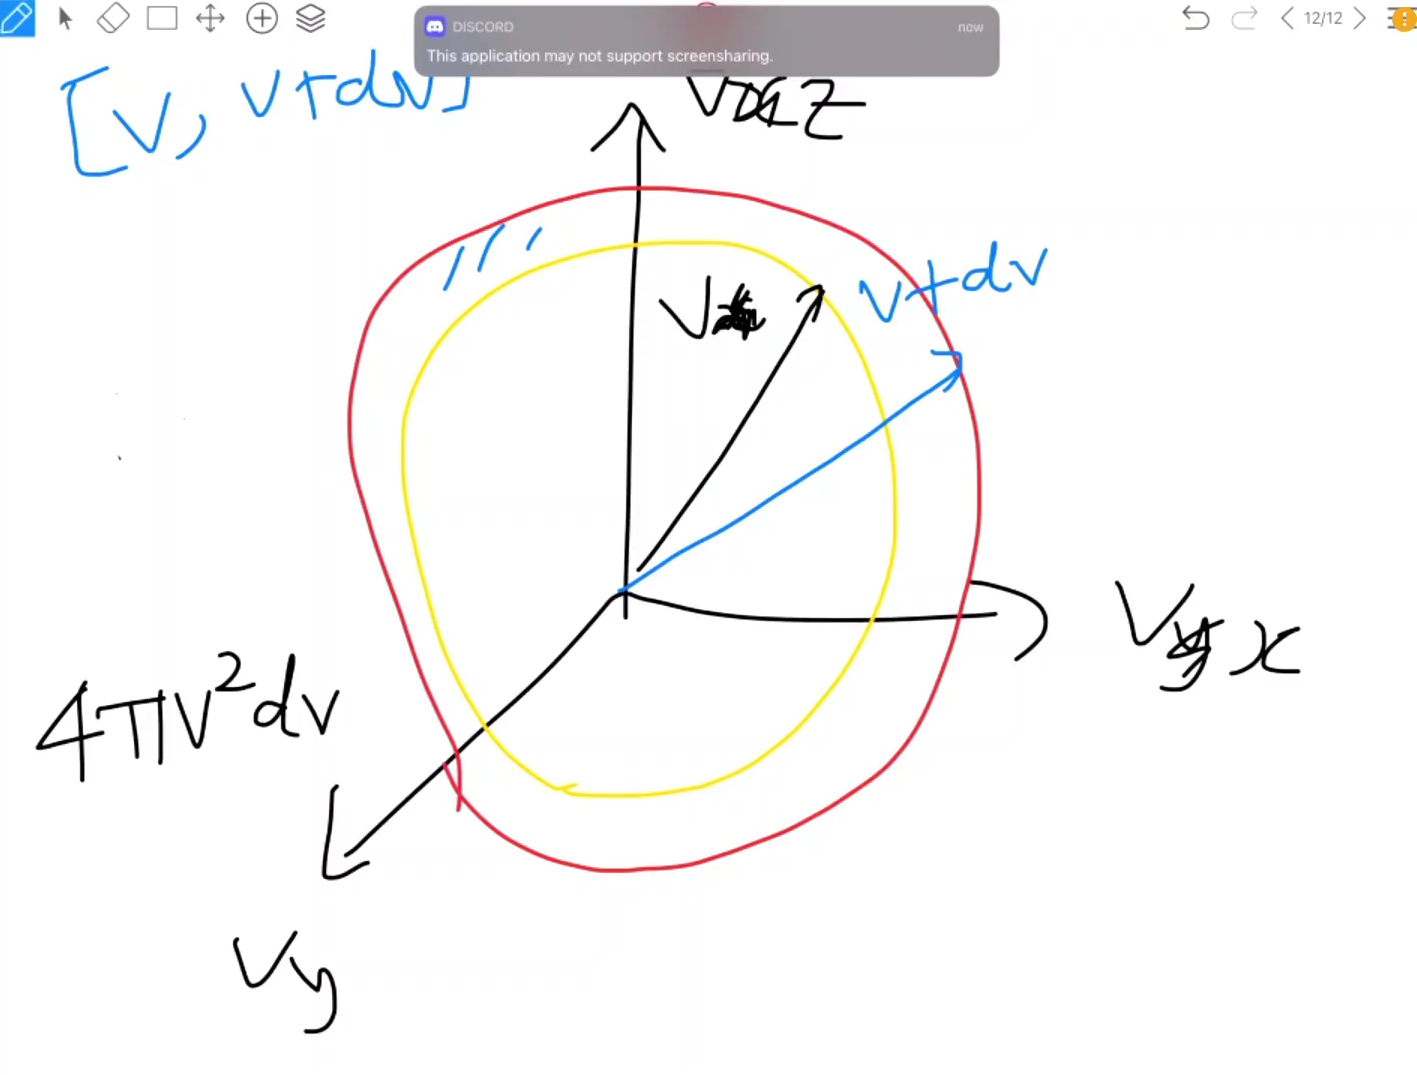
\includegraphics[width=0.5\linewidth]{velocity space.png}
    \caption{beautiful drawing by Ryan}
    \label{<label>}
\end{figure}
The volume enclosed, $V=4\pi v^2 dv$, between the red and yellow circle, multipled by the probability of the particles moving in that region, denotes the particles with speed $v \leq v_p \leq v+dv$. The speed probability distribution is then given by
\begin{equation}
    f(v)dv\propto v^2 \exp \bigg({\frac{-mv^2}{2k_B T}}\bigg)dv
\end{equation}

Integrating, we get
\begin{equation}
    f(v)=\frac{4}{\sqrt{\pi}}\bigg(\frac{m}{2 k_B T}\bigg)^\frac{3}{2} v^2 \exp\bigg({\frac{-mv^2}{2k_BT}}\bigg)
\end{equation}

Average speed:
\begin{equation}
    \langle v \rangle =\sqrt{\frac{8k_BT}{\pi m}}
\end{equation}

Root mean squared velocity: 
\begin{equation}
    \langle v^2 \rangle =\frac{3k_BT}{m} = \langle v_x^2\rangle + \langle v_y^2\rangle + \langle v_z^2\rangle
\end{equation}

Most probable speed: $df/dv=0$
\begin{equation} 
    v=\sqrt{\frac{2k_BT}{m}}
\end{equation}

Note: $m$ stand for the \textbf{mass of a single molecule}.

\subsection{Equipartition theorem}
Every degree of freedom will contribute $k_B T/2$ to the internal energy. 
\begin{equation}
    U=\frac{f}{2}k_BT
\end{equation}

More rigorous form: Each quadratic mode with energy in the form of $E=\alpha x^2$, where $x$ can be position or velocity, contributes $k_BT/2$ to the internal energy (so its not really about degree of freedom). It just so happens that both rotational and translational energy are $\propto v^2, \omega^2$

\section{How molecules move}
\subsection{Solid Angle}
In 2D, we have $s=r\theta$. In 3D, $A=r^2 \Omega$, where $\Omega$ is the solid angle (imagine the tip of the cone), and $A$ is the curved surface at the base of the cone. $\Omega \in [0,4\pi]$, as the maximum area subtended by a solid angle is that of a sphere: $A=4\pi r^2$

It is the same as if we have some angle $\theta$, and we increase by $d\theta$, the change in area on the spherical surface with unit length $1$ is $dA= 2\pi \sin \theta d\theta$. If we calculate with solid angle instead, where $\Omega \to \Omega + d\Omega$, $dA=(\Omega + d\Omega)r^2-\Omega r^2 = r^2 d \Omega$.
Hence, we obtain the \textbf{conversion factor} between $\Omega$ and $\theta$
\begin{equation}
    d\Omega=2\pi \sin \theta d\theta
\end{equation}

Imagine a bunch of particle being yeeted out from a point in all direction, the proportion of particle passing through a spherical cap with solid angle $d\Omega$ is $d\Omega/4\pi = \sin \theta d\theta/2$

\textcolor{blue}{\textit{There is a wall with area $A$. In time $dt$, what is the number of molecules that hit the wall that have $v \in [v,v+dv]$ and $\theta \in [\theta,\theta+d\theta]$.}}
Let $\rho_n$ be the volume number density, the number of molecules (per unit volume) that satisfy the condition (ignoring the wall)
\begin{equation}
    \rho_n f(v)\bigg(\frac{1}{2}\sin\theta\bigg)\,dv\,d\theta
\end{equation}
The number of particles that will hit the wall with area $A$ in time $dt$ would be 

\begin{equation}
    \rho_n f(v)\bigg(\frac{1}{2}\sin\theta\bigg)\,dv\,d\theta (A v \,dt \cos \theta )
\end{equation}
To find the number of particles hitting the wall \textbf{per unit area} and \textbf{per unit time}, we let $A$ and $dt$ be 1 (which is abit scam). The change in momentum experienced by those particles would then be 
\begin{align}
    dp &= (2mv \cos \theta)  \rho_n f(v)\bigg(\frac{1}{2}\sin\theta\bigg)\,dv\,d\theta v \cos \theta \\
    \textsf{Pressure} &= \int_{0}^{\infty}\int_0^{\frac{\pi}{2}}dp 
\end{align}
From here, you can derive the ideal gas equation: $pV=nRT$

\subsection{Ideal gas law}
\begin{equation}
    p=\frac{1}{3}\rho_n m \langle v^2 \rangle
\end{equation}
where $\rho_n$ is the number of molecules per unit volume. and $m$ is the mass of a single gas molecule.

\subsection{Molecular flux}
Molecular flux is the number of molecules striking the unit area per unit time (second). To calculate this, we just
\begin{align}
    \int_{0}^{\infty}\int_0^{\frac{\pi}{2}} &=\rho_n f(v)\bigg(\frac{1}{2}\sin\theta\bigg)\,dv\,d\theta \,v \cos \theta \nonumber \\
    \Phi &= \frac{1}{4}\rho_n \langle v \rangle = \frac{1}{4} \bigg(\frac{p}{kT}\bigg) \sqrt{\frac{8k_BT}{\pi m}}= \frac{p}{\sqrt{2\pi m kT}}
\end{align}
where molecular flux is usually denoted as $\Phi$. So if you have a box with a hole of area $A$ through which gas is allowed to escape, the number of molecules escaping per second would just be $N=\Phi A$. This process is called \textbf{Effusion}. Note that this formula only works if the area, $A$, is small. If $A$ is large, you will need to consider edge effects as the particles bouncing off some other surface can also escape through the hole. So, how small should the hole be? The condition is that 
\begin{equation}
    d \ll \lambda \, \textsf{, where $\lambda$ is the mean free path}
\end{equation}
The particle exiting from the small hole will \textbf{not} follow the Maxwell Boltzmann distribution becuase effusion is not a fair selection (if molecule is moving faster, it will have a higher chance of exiting the hole). 
\subsection{mean free path}
Mean free path is the average distance that a gas particle can travel before it collides with another particle. 

The mean collision time, $\tau$, is the average time that a gas particle takes to collide with another particle. We can define $\sigma$ as the cross-sectional area of the particle, and $P(t)$ as the probability of a particle \textbf{not} colliding up to a time $t$. 
\begin{align}
    P(t+dt)&=P(t)+\frac{dP}{dt}dt \nonumber \\
    &= \underbrace{P(t)}_{\textsf{Probability of not colliding up till $t$}} \times \underbrace{(....)}_{\textsf{probability of not colliding in $dt$}}
\end{align} 
In time $dt$, the particle will sweep a volume of $v\sigma dt$, and we want no molecule to be inside this volume. The probability of having a molecule inside this volume is $\rho_n v \sigma dt$, hence
\begin{equation}
    P(t)+\frac{dP}{dt}dt=P(t)\times\underbrace{(1-\rho_n v\sigma dt)}_{\textsf{probability of not colliding in $dt$}}
\end{equation}
We can just solve the differential equation by separation of variable and get the probability of a molecule not colliding up to time $t$ as
\begin{equation}
    P(t)=\exp(-\rho_n \sigma v t)
\end{equation}
Probability that it collides in the next $dt$ is 
\begin{equation}
    \underbrace{(e^{-\rho_n \sigma v t})}_{\textsf{not colliding up till $t$}} \times \underbrace{\rho_n \sigma v dt}_{\textsf{colliding in $dt$}} 
\end{equation}
Averaging it out across all time,
\begin{align}
    \langle t \rangle &= \int_0^{\infty}t(e^{-\rho_n \sigma v t})(\rho_n \sigma v dt) \nonumber \\
    \tau &= \frac{1}{\rho_n \sigma v}
\end{align}

However, we should instead use the relative speed, ${\langle v_r ^2 \rangle}$ instead of ${\langle v \rangle}$. Hence, the mean collision time, $\tau = 1/(\rho_n \sigma \sqrt{2}{\langle v \rangle})$ and mean free path, $\lambda={\langle v \rangle}\tau=1/(\sqrt{2}\rho_n\sigma)$

% Since $\lambda=\langle v\rangle \tau = \langle v_r \rangle/\rho_n \sigma v$ where $v_r$ is the relative speed. And according to maxwell boltzmann disribution, $\langle v \rangle \approx \sqrt {\langle v_r ^2 \rangle} \approx \sqrt{2} \langle v \rangle$

\section{First Law of thermodynamics}
The first law of thermodynamics state that:
\begin{equation}
    \Delta E= \Delta Q + W
\end{equation}
Since there is a plus sign in front of $W$, it must mean \textbf{work done on the gas}.
The differntial form of the the equation above is
\begin{equation}
    dE=dQ+dW
\end{equation}
where $dQ$ and $dW$ are called \textbf{inexact differential} since they are path dependent (and not state dependent)quantities.

On the other hand, $E$ is a state dependent quantity (depends on both temperature, $T$ and volume, $V$). Hence, a small change in $E$ ($dE$) can also be written as
\begin{equation}
    dE(T,V)=\bigg(\frac{\partial E}{\partial T}\bigg)_V dT+\bigg(\frac{\partial E}{\partial V}\bigg)_T dV
\end{equation}
\begin{mybox}{gray}{Molar specific heat at constant \textbf{volume} and \textbf{pressure}}
    Molar specific heat:
    \begin{itemize}
        \item at constant \textbf{volume}
              \begin{equation}
                  C_V=\bigg(\frac{\partial Q}{\partial T}\bigg)_V=\bigg(\frac{\partial E}{\partial T}\bigg)_V
              \end{equation}
              Proportionality factor between heat supplied and temperature change of a system at constant volume
        \item at constant \textbf{pressure}
              \begin{equation}
                  C_p
                  =\bigg(\frac{\partial Q}{\partial T}\bigg)_p
                  =\bigg(\frac{\partial (E-W)}{\partial T}\bigg)_p
                  =\bigg(\frac{\partial E}{\partial T}\bigg)_p+
                  p\bigg(\frac{\partial V}{\partial T}\bigg)_p
              \end{equation}
    \end{itemize}
    (the plus sign in front of the work is because $dQ=dE-dW$, and $dW=-pdV$. This is before when volume of gas decreases, work must be done \textbf{on} it, increasing its internal energy).
    \begin{flushleft}
        Since $\big(\frac{\partial V}{\partial T}\big)$ at constant pressure is essentially $\frac{nR}{p}$, the second term reduces to just $nR$.
    \end{flushleft}

    $$\boxed{\therefore C_p=C_V+nR}$$
    This shows that it takes more heat to increase temperature for an isobaric process. This is because extra energy is needed to offset those used when the gas does work by expanding.

    This relationship can actually be derived through many other methods as well. But just need to remember
    \textbf{first law of thermodynamics}, \textbf{internal energy's dependence on both temperature and volume}, as well as the fact that \textbf{heat capacity is a proportionality factor between heat input and change in temperature (internal energy)}, then shld be okay :)

\end{mybox}
\subsection{Quasi-static process}
\textbf{Definition}: A thermodynamic process that happens slowly enough for the system to remain in internal \textbf{thermodynamic equilibrium} (no tendency for the state of a system to change spontaneously).or in Ryan's words: a smooth curve on the $p-V$ diagram.
\subsubsection{Assuming a quasi-static process}
I think for most questions that talk about isochoric, isothermal and isobaric processes, the process is assumed to be quasi-static. This is because to be isothermal, isochoric or isobaric throughout the processes, you must be able to state the temperature, pressure and volume of the system at each step, which is possible only if the system is in equilibrium continuously.

\subsubsection{If process is not quasistatic}

If the question is about adiathermal process (according to Blundell, if the process is both adiathermal [without the flow of heat] and reversible, it's called adiabatic), the process can be carried out both quasi-statically and non quasi-statically. If the process is not quasi-static , we can no longer use the equation for various thermodynamic processes to solve the question. However, it is still possible to solve such questions using \textbf{conservation of energy.}

\begin{mybox}{green}{Quasi-static (reversible) process (my own interpretation)}
    If a gas changes state from A to B, it is only quasi-static if the intermediate states are all in thermodynamic equilibrium. Work done by isothermal / isochoric / isobaric processes are calculated with the assumption that processes are quasi-static (because infinitely small increments of change represent a continuous function).

    \begin{flushleft}
        E.g. If the process involves adding or removing weights from a piston (with gas beneath it), and the piston settles into a new equilibrium position, such a process is not quasi-static because the temperature / pressure / volume of the intermediate state is unknown (not in equilibrium). (Or when the process happens too fast such that there's insufficient time for the gas to settle into equilibrium)
    \end{flushleft}

\end{mybox}

\section{Second law of thermodynamics}
\subsection{Statements and Principles}
\subsubsection{Statements}
\begin{itemize}
    \item \textbf{Clausius' statement}: No process is possible whose \textbf{sole result} is the transfer of heat from a \textbf{colder to hotter} body. 
    \item \textbf{Kelvin-Planck statement}: No process is possible whose sole result is the complete conversion of heat into work, $Q_{\textsf{in}}\neq W$.
\end{itemize}

\subsubsection{Carnot Prciniple}
\begin{itemize}
    \item An irreversible heat engine is less efficient than a reversible one. \footnote{Proven by connecting a irreversible heat engine to a reversible one, and assuming it is more efficient. This will lead to a heat transfer from the cold reservoir to the hot reservoir, which violates Clausius' Statement.}
    \item Efficiencies of all reversible heat engines between identical heat reservoirs are the same. \footnote{Connect two reversible heat engines, A and B working in opposite directions. If A transfers from hot to cold and B transfers the other way, you will find that $\eta_A \leq \eta_B$. Swapping them will give $\eta_B \leq \eta_A$. We can conclude that $\eta_A=\eta_B$.}
\end{itemize}

\subsection{Conditions for reversibility}
\begin{itemize}
    \item Frictionless/Quasistatic
    \item Engine must have same temperature as reservoir.\footnote{Proven by connecting 2 reversible heat engines. The hot reservoir will gain net heat of $Q_H-Q_H=0$, same applies to the cold reservoir. By $0^{\textsf{th}}$ law of thermodynamics, they must be at the same temperature since there is no net heat transfer.} (Limit it to isothermal processes when exchanging heat, and adiabatic when not.)
\end{itemize}

Any reversible cycle working between 2 constant temperature heat reservoir should have the same efficiency as the \textbf{carnot engine}.

\subsection{Clausius Inequality}
\begin{mybox}{gray}{Clausius' inequality}
    Clausius' inequality states that for any closed loop,
    \begin{equation}
        \oint \frac{dQ}{T} \leq 0
    \end{equation}
    and equality must hold for reversible reactions.
    If the close loop consists of an irreversible, and an reversible part, we can write 
    \begin{equation}
        \int_A^B \frac{dQ}{T} + \int_B^A\underbrace{ \frac{dQ_{\textsf{rev}}}{T}}_{dS} \leq 0
    \end{equation}
    \begin{equation}
        dS\geq \frac{dQ}{T}
    \end{equation}
    In a thermally isolated system, $dQ=0$, and you will arrive at the second law of thermal dynamics: 
    \begin{equation}
        \boxed{dS\geq 0}
    \end{equation}
\end{mybox}

\subsection{Entropy}
Entropy is a state function (only dependent on initial and final states). For a \textbf{reversible process}, it is defined as such
\begin{equation}
    S(B)-S(A)=\Delta S= \int_A^B \frac{dQ_{\textsf{rev}}}{T}
\end{equation}

In general however,
\begin{equation}
    \Delta S \geq  \int_A^B \frac{dQ_{\textsf{irrev}}}{T}
\end{equation}

\textcolor{blue}{It is important to note that $\Delta S$ only depends on state, so it is the same regardless of whether the process is reversible or not.}

\subsubsection{Steps} {From this link: \href{https://www.physicsforums.com/insights/grandpa-chets-entropy-recipe/}{Entropy recipe}):
\begin{enumerate}
    \item Apply the First Law of Thermodynamics to the irreversible process to determine the final thermodynamic equilibrium state of the system
    \item Forget about the actual irreversible process, and focus instead exclusively on the initial and final thermodynamic equilibrium states.
    \item Devise a reversible path between the same two thermodynamic equilibrium states. This reversible path does not have to bear any resemblance whatsoever to the actual irreversible process path. \footnote{For example, even if the actual irreversible process is adiabatic, the reversible path you devise does not have to be adiabatic.  You can even separate various parts of the system from one another, and subject each of them to a different reversible path, as long as they all end up in their correct final states. Plus, there is an infinite number of reversible process paths that can take you from the initial state to the final state, and they will all give exactly the same value for the change in entropy.  So try to devise a path that is simple to work with (i.e., for which it is easy to apply step 3)}
    \item For the selected reversible path, evaluate the integral of $dQ/T$ from the initial state to the final state, where $aQ$ is the incremental amount of heat added to the system along the sequence of changes comprising the reversible path. ($\Delta S = \int dQ_\textsf{rev}/T$), where the subscript rev refers to the reversible path.
\end{enumerate}

\subsubsection{Entropy change of system with constant heat capacity, $C$}
\begin{equation}
    \Delta S = \int_{T_i}^{T_f} \frac{dQ}{T} =\int_{T_i}^{T_f} \frac{C dT}{T}= C\ln\bigg(\frac{T_f}{T_i}\bigg)
\end{equation}

\subsubsection{Expansion of ideal gas from $T_i, V_i \to T_f, V_f$}
\begin{equation}
    \begin{aligned}
        \Delta S = \int \frac{dQ}{T} =\int_{T_i}^{T_f} \frac{dU+pdV}{T} &= \int_{T_i}^{T_f} \frac{nC_V}{T} + \int_{V_i}^{V_f} \frac{nR}{V}dV \\
        &= nC_V \ln \bigg(\frac{T_f}{T_i}\bigg) + nR\ln \bigg(\frac{V_f}{V_i}\bigg)\\
    \end{aligned}
\end{equation}

\subsubsection{Joule Expansion}
This is equivalent to and isothermal Expansion from $V_i$ to $V_f$. 
\begin{equation}
    \Delta S = nR \ln \bigg(\frac{V_f}{V_i}\bigg)
\end{equation}

For an adiabatic process, $dQ=0$. Hence, there is no change in entropy for an adiabatic process (\textbf{isentropic})

\subsection{Fundamental Relations}

Going back to the first law of thermodynamics and let $dQ=TdS$ (only true for reversible reaction), we get
\begin{equation}
    dU=TdS-pdV
\end{equation}
All variables in this system are functions of state. $dS$ and $dV$ are extensive variables while $p$ and $T$ are intensive variables. If you scale up a sysem by 2 times, entropy and volume have to increase, while temperature and pressure can still remain the same.

\subsubsection{Spontaneity of process}
Let's say a system gains $dQ$ from environment, which has instantaneous temperature and pressure of $T_\textsf{ext}$ and $p_\textsf{ext}$,
\begin{equation}
    dS-\frac{dQ}{T_\textsf{ext}} \geq 0 \footnote{The LHS represents the entropy change of the universe(which is always positive), where $dS$ is the increase in entropy of the system. }
\end{equation}

Applying first law of thermodynamics, the following condition must be satisfied for process to be irreversible
\begin{equation}
    dQ=dU+p_\textsf{ext}dV+ T_\textsf{ext}dS \leq 0
\end{equation}
\begin{enumerate}
    \item \textcolor{blue}{Isolated system:} $dQ=0$, and $dS>0$ for spontaneous process.
    \item \textcolor{blue}{Solid:} $dV=0$, $dS=0$, and $dU<0$ for spontaneous process. 
    \item \textcolor{blue}{Constant $S$ and $p_\textsf{ext}$:} $dS=0$, $\Delta U + p_\textsf{ext} \Delta V=\Delta H <0$
    \item \textcolor{blue}{Constant $V$ and $T_\textsf{ext}$:} $dV=0$, $\Delta U - T_\textsf{ext} \Delta S=\Delta A <0$, where A is the \textbf{Helmholtz Free Energy}.
    \item \textcolor{blue}{Constant $p_\textsf{ext}$ and $T_{\textsf{ext}}$:} $\Delta (H-TS)=\Delta G<0$, where G is the \textbf{Gibbs Free Energy}.
\end{enumerate}

\section{Heat engines}
A Carnot engine (engine is defined as something that converts heat into work, 2 adiabats + 2 isotherms, cyclic process). We can prove by analysing each individual process that:
\begin{equation}
    \frac{Q_H}{Q_L}=\frac{T_H}{T_L}
\end{equation}

The analysis is as such: 

\begin{figure}[htbp]
    \centering
    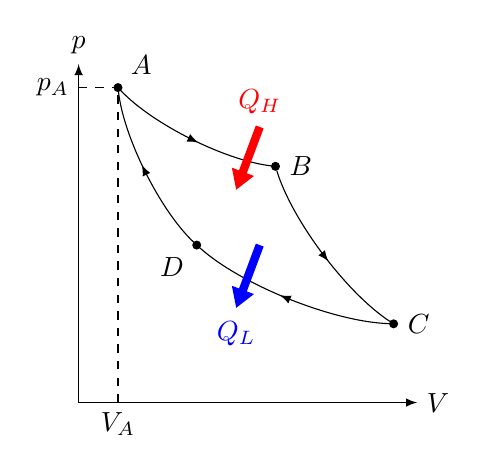
\begin{tikzpicture}[
        > = latex,
        dot/.style = {draw,fill,circle,inner sep=1pt},
        arrow inside/.style = {postaction=decorate,decoration={markings,mark=at position .55 with \arrow{>}}}
        ]
        \draw[<->] (0,4.3) node[above] {$p$} |- (4.3,0) node[right] {$V$};
        \node[dot,label={above right:$A$}] (@1) at (0.5,4) {};
        \node[dot,label={right:$B$}] (@2) at (2.5,3) {};
        \node[dot,label={right:$C$}] (@3) at (4,1) {};
        \node[dot,label={below left:$D$}] (@4) at (1.5,2) {};
        \draw[arrow inside] (@1) to[looseness=.7,bend right=20] (@2);
        \draw[arrow inside] (@2) to[looseness=.7,bend right=20] (@3);
        \draw[arrow inside] (@3) to[looseness=.7,bend left=20] (@4);
        \draw[arrow inside] (@4) to[looseness=.7,bend left=20] (@1);
        \draw[dashed,thin] (0,4) node[left] {$p_A$} -- (0.5,4);
        \draw[dashed,thin] (0.5,0) node[below] {$V_A$} -- (0.5,4);
        \draw[red, fill=green, -{Triangle[width = 8pt, length = 7pt]}, line width = 3pt] (2.3, 3.5) node[above] {$Q_H$} -- (2.0, 2.7);
        \draw[blue, fill=green, -{Triangle[width = 8pt, length = 7pt]}, line width = 3pt] (2.3, 2) -- (2, 1.2) node[below] {$Q_L$};
    \end{tikzpicture}
    \caption{Carnot engine. $AB$ and $CD$ are isotherms, while $BC$ and $DA$ are adiabats. $AB$ is maintained at constant temperature $T_H$, while $CD$ is maintained at constant temperature $T_L$.}
    \label{carrot}
\end{figure}

\begin{enumerate}
    \item $\boxed{A\to B}$, $Q_H=nRT_H \ln(V_B/V_A)$
    \item $\boxed{B \to C}$, $T_H/T_L=(V_C/V_B)^{\gamma-1}$
    \item $\boxed{C \to D}$, $Q_L=-nRT_L \ln(V_D/V_C)$
    \item $\boxed{D \to A}$, $T_L / T_H=(V_A/V_D)^{\gamma-1}$
\end{enumerate}

Efficiency a carnot engine (turns heat into work) is defined as the ratio of work done to the heat input,

\begin{equation}
    \eta=\frac{W}{Q_H}=\frac{Q_H-Q_L}{Q_H}=1-\frac{T_L}{T_H}
\end{equation}. 

The reason why $W=Q_H-Q_L$ is because the process is cyclic and there is no change in internal energy.

\begin{flushleft}
    However, for a refrigerator (engine run in reverse), the efficiency is defined as a different way. It is instead
    \begin{equation}
        \eta=\frac{Q_L}{W}
    \end{equation}
    It makes sense because efficiency in this case means the amount of heat you can \textbf{remove} from a refrigerator when the engine does a certain amount of work. (similar for a heat pump, where the engine does work to pump heat instead of remove heat).
\end{flushleft}

\chapter{Fluid for sypt 2023 :)}
Stuff from Fox and McDonald's introduction from fluid dynamics in the
\section{Eulerian}
In fluid dynamics, it is common to use the Eulerian method of description, which focuses attention on the properties of a flow at a given point in space as a function of time. For example $v(x,y,z,t)$.
\chapter{Special Relativity}
There are 3 fundamental effects of special relativity
\begin{itemize}
    \item Loss of simultaneity
    \item Time dilation
    \item Length contraction
\end{itemize}
\section{kinematics}
Let the frame $S'$ be moving at speed $v$ relative to a stationary frame $S$. Denote all quantities (for e.g. time) in the $S'$ frame with a prime ($'$).  
\subsection{basics}
\textbf{Time dilation}
\begin{equation}
    t'=\frac{t}{\gamma}
\end{equation}
\textbf{Length contraction}
\begin{equation}
    \ell'=\frac{\ell}{\gamma}
\end{equation} \footnote{$t'$ and $\ell'$ are the time and length in the moving frame $S'$.}
where $\gamma=1/\sqrt{1-\frac{v^2}{c^2}}$
Since $c$ is the maximum possible speed a thing can reach, $\gamma$ will always be \textbf{greater than or equal to} 1. 
\subsection{Lorentz transformation}
When $S'$ is moving in the positive $x$ direction relative to $S$, the Lorentz transformation is written as follows: 

\begin{multicols}{2}
    \begin{equation}
        \begin{bmatrix}
            ct' \\
            x'
        \end{bmatrix}
        =
        \begin{bmatrix}
            \gamma & -\beta \gamma \\
            -\beta \gamma & \gamma 
        \end{bmatrix}
        \begin{bmatrix}
            ct\\
            x 
        \end{bmatrix}
    \end{equation}\break


    \begin{equation}
        \begin{bmatrix}
            ct \\
            x
        \end{bmatrix}
        =
        \begin{bmatrix}
            \gamma & \beta \gamma \\
            \beta \gamma & \gamma 
        \end{bmatrix}
        \begin{bmatrix}
            ct'\\
            x'
        \end{bmatrix}
    \end{equation}
\end{multicols}

This is lorentz transformation in the matrix form, where the transformation matrix is known as the \textbf{lorentz boost}. \textcolor{blue}{To boost from the $S$ frame to the $S'$ frame, we have the "$-$" sign. To boost from the $S'$ frame to the $S$ frame, we have the "$+$" sign.}


\begin{equation}
    \begin{cases}
      \Delta x= \gamma (\Delta x' + v \Delta t') \\
      \Delta t= \gamma (\Delta t'+v \frac{\Delta x'}{c^2})\\
    \end{cases}      
\end{equation} 

\begin{equation}
    \begin{cases}
      \Delta x'= \gamma (\Delta x - v \Delta t) \\
      \Delta t'= \gamma (\Delta t - v \frac{\Delta x}{c^2})\\
    \end{cases}      
\end{equation} 

To derive the equation for time dilation, we note that the person measuring it (either in $S$ or $S'$) has to be stationary (i.e. $v=0$).

From the equation above and setting $\Delta x'$ to 0, we see that $\Delta t=\gamma \Delta t'$. Since $\gamma\geq 1$, the time elapsed measured by the stationary observer in the $S'$ frame is always shorter than the time elapsed in $S$. 

However, if we set $\Delta x$ to 0 and use the second set of equation, we get $\Delta t'=\gamma \Delta t$. This seems to be a contradiction. But in fact, this scenario is very different as the stationary observer is now in the $S$ frame (and not the $S'$ frame).

\subsection{relativistic velocity addition}
Let $v_1$ be the speed of the object measured in the frame $S'$, which is moving at speed $v_2$ relative to the ground.

Writing out the lorentz transformation for $S'$, we get 

\begin{equation}
    \begin{cases}
        \Delta x= \gamma_2 (\Delta x'+v_2 \Delta t')\\
        \Delta t = \gamma_2 (\Delta t'+v_2 \frac{\Delta x'}{c^2})\\
    \end{cases}
\end{equation}
where $\gamma_2$ is the Lorentz factor associated with $v_2$.
As the speed measured in the lab frame ($S$) is defined as $\Delta x/\Delta t$, we get 
\begin{equation}
    \frac{\Delta x}{\Delta t}= \frac{\gamma_2 (\Delta x'+v_2 \Delta t')}{\gamma_2 (\Delta t'+v_2 \frac{\Delta x'}{c^2})} = \frac{v_1+v_2}{1+(v_1 v_2)/c^2}
\end{equation}
The derivation \textbf{above} only applies to velocity addition in the \textbf{longitudinal direction}. For \textbf{transverse velcoity addition}, we can use a similar method (Lorentz transformation: $\Delta y'=\Delta y= v \Delta t $)
\begin{equation}
    \frac{\Delta y}{\Delta t}=\frac{\Delta y'}{\gamma (\Delta t'+v \frac{\Delta x'}{c^2})} =\frac{\Delta y'/\Delta t'}{\gamma (1 +v \frac{\Delta x'/\Delta t'}{c^2})}= \frac{v_y'}{\gamma (1+v'_x\frac{v}{c^2})}
\end{equation}

Now, let's derive this result with \textbf{4-vectors}. The velocity 4-vector, $V^\mu$, is
\begin{equation}
    V^\mu = (\gamma_{v_1} c, \gamma_{v_1} \vec {v_1})
\end{equation}
Setting $c=1$ so that our equations do not get too messy, $V^\mu_{S'}=(\gamma_{v_1}, \gamma_{v_1}, 0,0)$ in $S'$. In $S$, $V^\mu_S = (\gamma_w, \gamma_w w, 0,0)$, where $w$ is the speed of the object in $S$ frame. Using the fact that \textbf{inner dot product of 4-vector is invariant across all reference frames}\footnote{In general, the inner dot product of 4 vectors, $K^\mu W_\mu=K_0W_0-K_1W_1-K_2W_2-K_3W_3$}, we can write
\begin{equation}
    V^\mu_{S'} \cdot V_{\mu,S'} = V^\mu_S \cdot V_{\mu,S}.
\end{equation}
Solving for $w$, we should get the same answer. 

\subsection{invariance and minkowski diagram}
Consider the quantity $(\Delta s)^2= c^2(\Delta t)^2- (\Delta x)^2$, where $s$ (dropping the $\Delta$ from now on) is known as the \textbf{invariant interval} because this quantity is invariant to coordinates (i.e. $ct-x=ct'-x'$, $(ct, x)$ is usually known as the \textbf{spacetime interval}). 

\begin{figure}[H]
    \centering
    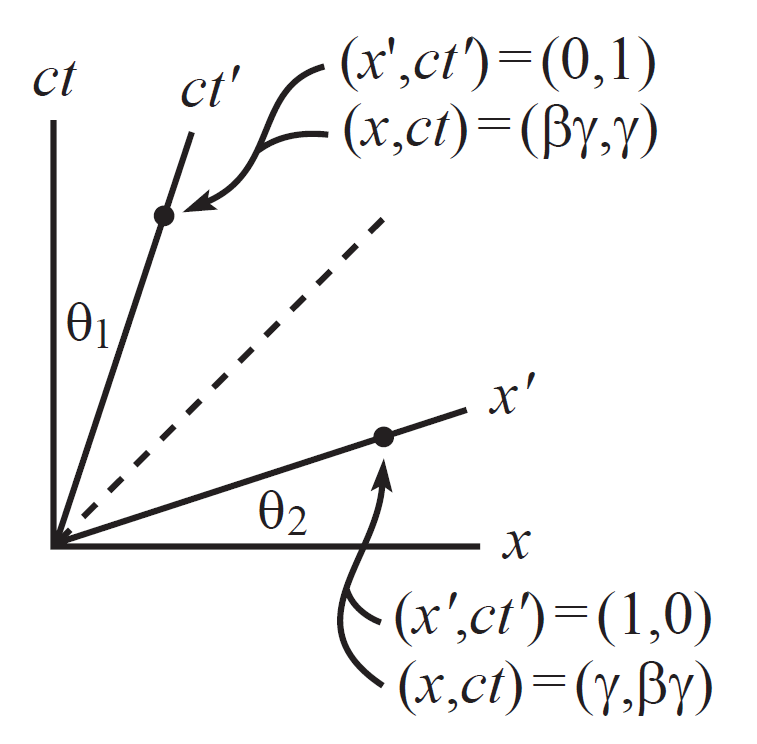
\includegraphics[width=0.3\textwidth]{minkowski.png}
\end{figure}
This could be derived with \textbf{lorentz transformation} with $\beta =v/c$. 1 unit on the $ct$ axis would correspond to $\gamma\sqrt{(1+\beta^2)}$ on the $ct'$ axis. Hence,
\begin{equation}
    \frac{\textsf{one} \ ct' \ \textsf{unit}}{\textsf{one} \ ct \ \textsf{unit}}=\frac{\sqrt{1+\beta^2}}{\sqrt{1-\beta^2}}
\end{equation}

Simultaenous measurements can be represented by drawing a line perpendicular to the $ct$/$ct'$ axes and seeing the points of intersection of the line with the $ct$/$ct'$ axes. 

\section{dynamics}
\subsection{Energy and momentum}
\textbf{Energy}
\begin{equation}
    E=\gamma m c^2
\end{equation}
\textbf{Momentum}
\begin{equation}
    \mathbf{p}=\gamma m \mathbf{v}
\end{equation}
To justify these expressions, I think it is quite elegant to perform Taylor series expansion in the limit of $v \ll c$ for $1/\sqrt{1-x^2}$ \footnote{$(1+x)^{-\frac{1}{2}}=1-\frac{1}{2}x+\frac{3}{8}x^2-\frac{5}{16}x^3+\frac{35}{128}x^4...$}, you obtain

\begin{equation}
    \begin{cases}
        E=mc^2(1+\frac{1}{2}(\frac{v}{c})^2+\frac{3}{8}(\frac{v}{c})^3+\frac{5}{16}(\frac{v}{c})^4+...)=mc^2+\frac{1}{2}mv^2+...\\
        \mathbf{p}=m \mathbf{v}(1+\frac{1}{2}(\frac{v}{c})^2+\frac{3}{8}(\frac{v}{c})^3+\frac{5}{16}(\frac{v}{c})^4+...)=m\mathbf{v}+...\\
    \end{cases}
\end{equation}

There is this very important equation
\begin{equation}
    E^2=p^2c^2+m^2c^4
\end{equation}
Another pretty useful equation is from the fundamental equations describing relativistic momentum and energy, 
\begin{equation}
    \frac{\mathbf{p}}{E}=\frac{\mathbf{v}}{c^2}
\end{equation}

Moreover, the equations to convert energy and momentum between frames are also quite elegant. Let the particle be travelling at speed $v$ in frame $S'$, which is moving at speed $u$ relative to lab frame $S$, then the energy and momentum in the 2 frames are related through
\begin{equation}
    \begin{cases}
        E=\gamma_u(E'+vp')\\
        p=\gamma_u(p'+vE')\\
    \end{cases}
\end{equation} \footnote{$E'=\gamma_v m$ and $p'=\gamma_v m v$, note that it is $\gamma_v$ and not $\gamma_u$}

Through this equation, we note that $E$ and $p$ behave exactly the same way as $ct$ and $x$. Hence, we obtain the following equation
\begin{equation}
    m^2=E^2-p^2=E'^2-p'^2
\end{equation}
where the mass of the particle, $m$, is the \textbf{invariant quantity}.

\subsection{Relativistic Collisions}
It is important to note that this $E=\gamma mc^2$ here is not equivalent to kinetic energy($E-mc^2$). During collision, it is the \textbf{total energy} that is conserved, so always use $E$ and not KE. 

To solve collisions problems, it is nice to define a \textbf{4- momentum}, or $P=(E,p_x,p_y,p_z)$ \footnote{Note that it shld be $E/c$ to make it dimensionally consistent but since $c=1$, we can just write it like this}. The inner product of this "vector" is defined to be $a_1b_1-a_2b_2-a_3b_3-a_4b_4$. It is defined this way so that we can concisely write $m^2=E^2-p^2$ as 
\begin{equation}
    P\cdot P=m^2
\end{equation}

\subsection{Optimal Collisions}
The minimum energy configuration of a system of particles with fixed total momentum is the one where they all move with the same velocity. This is easiest to show by boosting to the center of mass frame (i.e. the frame with zero total momentum) and then boosting back.


\subsection{Force}






\section{4-vector}
The most basic 4-vector is the \textbf{4-displacement} between two points in spacetime, which we call events. The 4-displacement is a fundamentally invariant geoemtric object, which you can think of as an arrow pointing between these 2 events. 

Consider two inertial frame $S$ and $S'$, such that $S'$ is moving at speed $v$ in the positive x-direction relative to $S$. Their coordinates are calibrated such that their origins coincide at $t=t'=0$. The frames are said to be in \textbf{standard configuration}, and their change-of-coordinates transformation can be summarised by the following
\begin{equation}
    \begin{bmatrix}
        ct' \\
        x' \\ 
        y' \\ 
        z'
    \end{bmatrix}
    =
    \begin{bmatrix}
        \gamma & \beta \gamma &  & \\
        -\beta \gamma & \gamma &  & \\ 
         &  & 1 & \\ 
         &  &  & 1
    \end{bmatrix}
    \begin{bmatrix}
        ct\\
        x \\ 
        y \\ 
        z
    \end{bmatrix}
\end{equation}



\chapter{Math}
\section{Single variable calculus}
\section{Multi-variable calculus}
\subsection{Why does gradient points in direction of greatest ascent}
\begin{mybox}{green}{Intuition - Explanation 1}
    Easy explanation (imo): "Gradient" is defined as the vector summation of
    \begin{equation}
        \nabla{f}=\frac{\partial f}{\partial x} \hat{i}+\frac{\partial f}{\partial y}\hat{j}+ .....
    \end{equation}
    the maximum rate of change along the individual axes. So naturally, the summation of these rate of changes would give the maximum rate of change as well.
\end{mybox}

\begin{mybox}{green}{Intuition/Proof - Explanation 2 (by \textbf{Yi Fan})}
    Single variable tangent line approximation:
    \begin{equation}
        f(x)\approx f(x_0)+ f'(x_0)(x-x_0)
    \end{equation}

    Multi-variable (2 in this case) tangent \textbf{plane} approximation:
    \begin{equation}
        f(x,y)-f(x_0,y_0) \approx f_x(x_0,y_0)(x-x_0) + f_y(x_0,y_0)(y-y_0)
    \end{equation}
    where $f_x$ and $f_y$ denotes partial derivatives with respect to $x$ and $y$ respectively.

    \begin{flushleft}
        Locally if we zoom in near $(x_0, y_0)$ this shows that any nice function is just a plane.
    \end{flushleft}
    \begin{flushleft}
        Then now suppose our plane is given by $z = ax + by$, where we take reference point to be the origin (otherwise we can just translate the function).
    \end{flushleft}
    \begin{flushleft}
        Now you can think of it as $z = (a,b)\cdot (x,y)$ where we have a dot product, and we want to find the direction $(x,y)$ that maximises this. ($a = f_x(x_0, y_0)$ and $b = f_y(x_0,y_0)$)
    \end{flushleft}
    \begin{flushleft}
        But dot product is maximised when the vector points in parallel direction. So we must have $(x,y) = k(a,b)$ for some constant $k$.
    \end{flushleft}
    \begin{flushleft}
        So essentially, we are trying to move $(x,y)$ around such that we can get the maximum $z$ value. And we realised that when $(x,y)$ is aligned with the gradient, the maximum $z$ value is achieved. Hence, \textbf{gradient always points in direction of greatest ascent.}
    \end{flushleft}

\end{mybox}

\subsection{Divergence}
\subsection{Curl}

\section{Differential equations}
\subsection{Linear differential equations - from Hexiang's slides}
If you want to solve something simple like
$$\frac{dy}{dx}=ay,$$
one could use separation of variables
$$\int dx=\frac{1}{a}\int \frac{1}{y} dy$$
$$x+d=\frac{\ln(y)}{a}+c$$
$$ax+c=\ln(y)$$
$$y=e^{ax+c}=e^{ax}e^c$$
which can be generalised to
$$y=Ae^{ax}.$$
Alternatively, we can also guess some solution, maybe $y=e^{cx}$ will do. $\frac{dy}{dx}=ce^cx$. Hence, $c=a$. This solution wil still hold true when we multiply it by an arbitrary constant ($y=Ae^{ax}$).

\subsection{Solution to $\ddot x=-\omega^2 x$}
Let's try subbing in $x=Ae^{ct}$ again and see what we get,
$$\ddot x= c^2 A e^{ct}$$
$$c^2 A e^{ct}=-\omega^2 Ae^{ct}$$
$$c=\pm i\omega$$
So there are 2 possible values for $c$, hence 2 solutions for $x$ ($Ae^{i\omega t}$ or $Ae^{-i\omega t}$)
For a linear differential equation (in this case it is), the most general solution would be the \textbf{linear combination} of the individual solutions
$$\boxed{x=A_1 e^{i\omega t} + A_2 e^{-i\omega t}}$$
Using \textbf{Euler's identity}
$$x=A_1(\cos(\omega t)+i \sin(\omega t))+A_2(\cos(-\omega t)+i \sin(-\omega t))$$
$$x=(A_1+A_2)\cos(\omega t)+i(A_1-A_2) \sin(\omega t)$$
$$x=B\cos(\omega t)+C\sin(\omega t)$$
which can then be converted to the form which we are more familiar with (r-formula): $$\boxed {x=A\sin(\omega t + \phi) \quad \textsf{or}\quad x=A\cos(\omega t + \phi).}$$ Since we absorbed $i$ into the constants, $A$ and $\phi$ are both complex right now. However, we can just impose the conditions that they must always be real for physical purposes.
\subsection{Integrating fractor}
If you have an equation in the form of

\begin{align}
    \frac{dy}{dx}+P(x)y &= Q(x)\\
    M(x)\frac{dy}{dx}+M(x)P(x)y &= M(x)Q(x)\\
\end{align}

You can multiply both side by an integrating factor $M(x)$, such that the LHS becomes the result of a product rule. This is useful because once we can get it to be like product rule, we can integrate both side and solve for $y$.

\begin{align}
    M(x)y &= \int Q(x)M(x)dx\\
    y &= \frac{\int Q(x)M(x)dx}{y}
\end{align}

How do we find this integrating factor?

\begin{equation}
    M'(x)=M(x)P(x)
\end{equation}

\begin{equation}
    \boxed{M(x)=\exp\bigg(\int P(x)dx \bigg)}
\end{equation}

\section{Cool integrals}
\subsection{Gaussian integral}
\begin{equation}
    \int_{-\infty}^\infty e^{-x^2}dx=\sqrt{\pi}
\end{equation}

\begin{equation}
    \int_{-\infty}^\infty e^{-\alpha x^2}dx=\sqrt{\frac{\pi}{\alpha}}
\end{equation}
Very useful in thermodynamics. 
\chapter{PO training}

\section{18/08/22}
\subsection{Gallilean Invariance}
All things in newtonian physics has to obey \textbf{gallilean invariance}, meaning that the laws have to hold true in every inertial reference frame (i.e. stationary frame/frame moving at constant $v$)

In school, we are taught that since $\mathbf{F}=\frac{d\mathbf{p}}{dt}$ where $\mathbf{p}=m \mathbf{v}$, by chain rule, we will get 

\begin{equation}
    \mathbf{F}=\frac{d (m\mathbf{\vec{v}})}{dt}=m\frac{d\mathbf{v}}{dt}+\mathbf{v} \frac{dm}{dt}
\end{equation}

Now, we shall verify the galliean invariance of the equation above. Let's have a frame $S'$ moving at constant velocity $\mathbf{u}$. The force, mass,velocity and time in $S'$ are denoted with a prime ($'$). Note that this frame is \textbf{inertial} and \textbf{all newtonian laws should hold in inertial frames}.

\begin{align}
    \mathbf{F}'=m'\frac{d\mathbf{v'}}{dt'}+\mathbf{v'} \frac{dm'}{dt'}
\end{align}

Since mass time and force are invariant, and $\mathbf{v'}=\mathbf{v}-\mathbf{u}$, we can rewrite it as 
\begin{equation}
    \mathbf{F}=m\frac{d\mathbf{v}}{dt}+(\mathbf{v}-\mathbf{u})\frac{dm}{dt}
\end{equation}
which is definitely not the same as the equation above. Hence, it is proven that the equation 7.1 is \textbf{not} gallilean invariant.

\subsection{rocket momentum}
However, in some special cases, the "wrong" equation can still be applied. 
Let the mass and velocity of a rocket be $m(t)$ and $v(t)$ respectively. 
At time $t'=t+\Delta t$
\begin{align}
    m(t)v(t) 
    &= m(t')v(t')+ (m(t')-m(t))(v(t')-u)\\
    &= (m(t)+\Delta m)(v(t)+\Delta v)+(-\Delta m)(v(t)+\Delta v - u)
\end{align}

where $u$ is the speed of the fuel (particle) emitted.

Expanding the equation, we get
\begin{equation}
    m(t)v(t)=m(t)v(t)+m(t)\Delta v+\Delta m v(t)+\Delta m \Delta v -\Delta m v(t)-\Delta m \Delta v - \Delta m u 
\end{equation}

Simplifying everything, we get 
\begin{equation}
    m dv+u dm = 0
\end{equation}

\section{25/08/22}
\subsection{linear independence of solution}
From wikipedia: A sequence of vectors $\mathbf{v_1},\mathbf{v_2},...\mathbf{v_k}$ from a vector space $V$ is said to be \textbf{linearly dependent} if there exist scalars $a_1,a_2,...,a_k$, not all zero, such that 
\begin{equation}
    a_1 \mathbf{v_1}+a_2 \mathbf{v_2}+...+a_k \mathbf{v_k}= \mathbf{0}
\end{equation}
where $\mathbf{0}$ denotes the zero vector. 
basically, as long as the vectors are not parallel, they are \textbf{linearly independent}

\section{27/08/22}
\subsection{Newton-Raphson method}
for example if you wanna solve
\begin{equation}
    y=f(x)=0
\end{equation}
you can kinda use
\begin{equation}
    x_{n+1}=x_n-\frac{f(x_n)}{f'(x_n)}
\end{equation}

 but its kinda useless

 \subsection{PS 2 Q 7}
 how to decide the direction of static friction? do torque about the contact point (where static friction acts), and realise that torque by $F$ has to result in a clockwise rotation (into the page). This means that torque about the COM also has to be clockwise, meaning that static frction points in the opposite direction of $F$. 

\textbf{Kenneth Hong's solution}
Translational motion of the center of mass
\begin{equation}
    F \cos \theta - f_s= ma_{CM,x}
\end{equation}
Rotational mostion about the centre of mass $I=M(a^2+b^2)/2$
\begin{equation}
    f_s a - Fb=I\alpha
\end{equation}

with the additional no slip condition ($a_{CM,x}=a\alpha$) and solving for pure rolling, you get
\begin{equation}
    \begin{cases}
        a_{CM,x}=\frac{F/M}{1+I/Ma^2}(\cos\theta-\frac{b}{a})\\
        f_s=\frac{F}{1+I/Ma^2}(\frac{I}{Ma^2}\cos\theta+\frac{b}{a})
      \end{cases}
\end{equation}

Maximum tension:
\begin{equation}
    f_s \leq \mu_s (Mg-F \sin\theta)
\end{equation}
\begin{equation}
    T_{max}=\frac{\mu_s (1+I/Ma^2)/Mg}{(I/Ma^2)\cos\theta+\mu_s(1+I/Ma^2)\sin\theta+b/a}
\end{equation}

\subsection{PS 2 Q 8}

\indent Workdone by friction on a rolling and \textbf{slipping} object is not just $W=f_k \cdot d$, where $d$ is the displacement of the centre of mass.

It is actually
\begin{align}
    W_{f_k} 
    &= W_{\textsf{trans}}+W_{\textsf{rot}}\\
    &= \int_0^{\Delta x} f_k dx - \int_0^{\Delta \theta} \tau d \theta 
\end{align}

Note that it is a minus sign because in the question, friction is adding energy in the translational motion, but removing energy in the rotational motion. 


\chapter{Quantum Mechanics}
This part is written after I graduated from Junior College in 2023. 

\section{Schrodinger Equation}

\subsection{Time-independent}
\begin{equation}
    \hat{H}\Psi = E\Psi
\end{equation}

\textbf{Hilbert Space:} The set of all square-integratable functions (mathematicians call it $L_2$). All wave-functions live in the Hilbert space. 

The expectation value of an observable $Q(x,p)$ can be expressed in the inner product notation as 

\begin{equation}
    \langle Q \rangle = \langle \Psi^{*} | \hat{Q} \Psi \rangle.
\end{equation}
Because $Q$ represents a real observable, it does not have an imaginary part and hence $\langle Q\rangle ^*=\langle Q\rangle$.

\begin{equation}
    \langle Q\rangle=\langle Q\rangle^* \longrightarrow  \langle \Psi | \hat{Q} \Psi \rangle = \langle \hat{Q} \Psi | \Psi \rangle.
\end{equation}
An operator with such a property is known as a $\textbf{Hermitian Operators}$.

The hermitian conjugate of an operator $\hat{Q}$ is defined as $\hat{Q}^\dagger$ such that: 
\begin{equation}
    \langle \Psi | \hat{Q} \Psi \rangle = \langle \hat{Q}^\dagger \Psi | \Psi \rangle.\footnote{For a hermitian operator, $\hat{Q}=\hat{Q}^\dagger$.}
\end{equation}

An observable $Q$ subject to some wavefunction $\Psi$ will not always return the same value (although the mean is always $\langle \Psi \rangle$). However, there exists wave functions $\Psi$ that produce the same value $q$ for all measurements of $Q$. Such functions are known as \textbf{determinate states}. 
\begin{CJK*}{UTF8}{gbsn}
\chapter{China physics insane}

\section{电磁}
\subsection{CP 对称性}
C 代表 charge,P 是 position。电偶极矩(vector quantity)的镜像 (about a plane)跟它一样 (因为不光电极相反,正负电核的位置也相互交换)。单独电核的话量一样大但是极却相反。

\section{信息熵}
\begin{equation}
    S=k \sum_{i=1}^{n} -p_i \ln (p_i)
\end{equation}


\end{CJK*}

\end{document}
